\chapter{Nonprompt Background Estimation}
\label{chap:Nonprompt}

In this analysis, the term \emph{prompt} leptons refers to leptons that originate from the \ac{CLFV} vertex, the \ac{DY} process, or an electroweak boson decay, including leptons from $\uptau$ decays if the $\uptau$ lepton originates from the latter two processes. \emph{Nonprompt} leptons refer to leptons that originate from hadron decays and photon conversions, as well as particles misidentified as leptons. \emph{Nonprompt} leptons are suppressed through isolation requirements and a \ac{MVA}-based identification specifically trained to reject them.

\emph{Nonprompt} backgrounds are defined to be backgrounds with at least one \emph{nonprompt} lepton passing the \emph{tight} selection criteria, in this case generally dominated by \ac{DY} and $\ttbar$ production. An accurate estimation of \emph{nonprompt} backgrounds is difficult to achieve through \ac{MC} modeling. Therefore, a data-driven technique called the ``\mm'' \cite{Gillam:2014xua} is used to estimate the \emph{nonprompt} backgrounds. 

A brief description of the \mm~in its simplest form is given in \autoref{sec:MM} followed by its generalization and implementation in \autoref{sec:MR}. This method is validated using three \acp{VR} and is described in \autoref{sec:VR}. Lastly, the \emph{nonprompt} estimation in the \ac{SR} is presented in \autoref{sec:MMSR}.
%%%%%%%%%%%%%%%%%%%%%%%%%%%%%%%%%%%%%%%%%%%%%%%%%%%%%%%%
%%%%%%%%%%%%%%%%%%%%%%%%%%%%%%%%%%%%%%%%%%%%%%%%%%%%%%%%

\section{The Matrix Method}
\label{sec:MM}

The \mm~is a data-driven technique used to estimate the fraction of \emph{nonprompt} leptons that pass a given lepton selection, referred to as ``\emph{tight}''. The \emph{tight} selection usually incorporates tight lepton identification and isolation requirements and corresponds to the full lepton selection used in an analysis. The \emph{loose} selection is obtained by loosening the \emph{tight} selection. The \emph{loose} selection is used as a baseline such that any \emph{loose} leptons fall into one of the two exclusive categories: \emph{tight} or \emph{not tight}. The \mm~deals with \emph{prompt} and \emph{nonprompt} leptons separately. As a result, \emph{prompt} and \emph{nonprompt} efficiencies are introduced, as illustrated in Figure~\ref{fig:Matrix_Method}.

 \begin{figure}[tbh!]
 \begin{center}
 \begin{tabular}{c}
 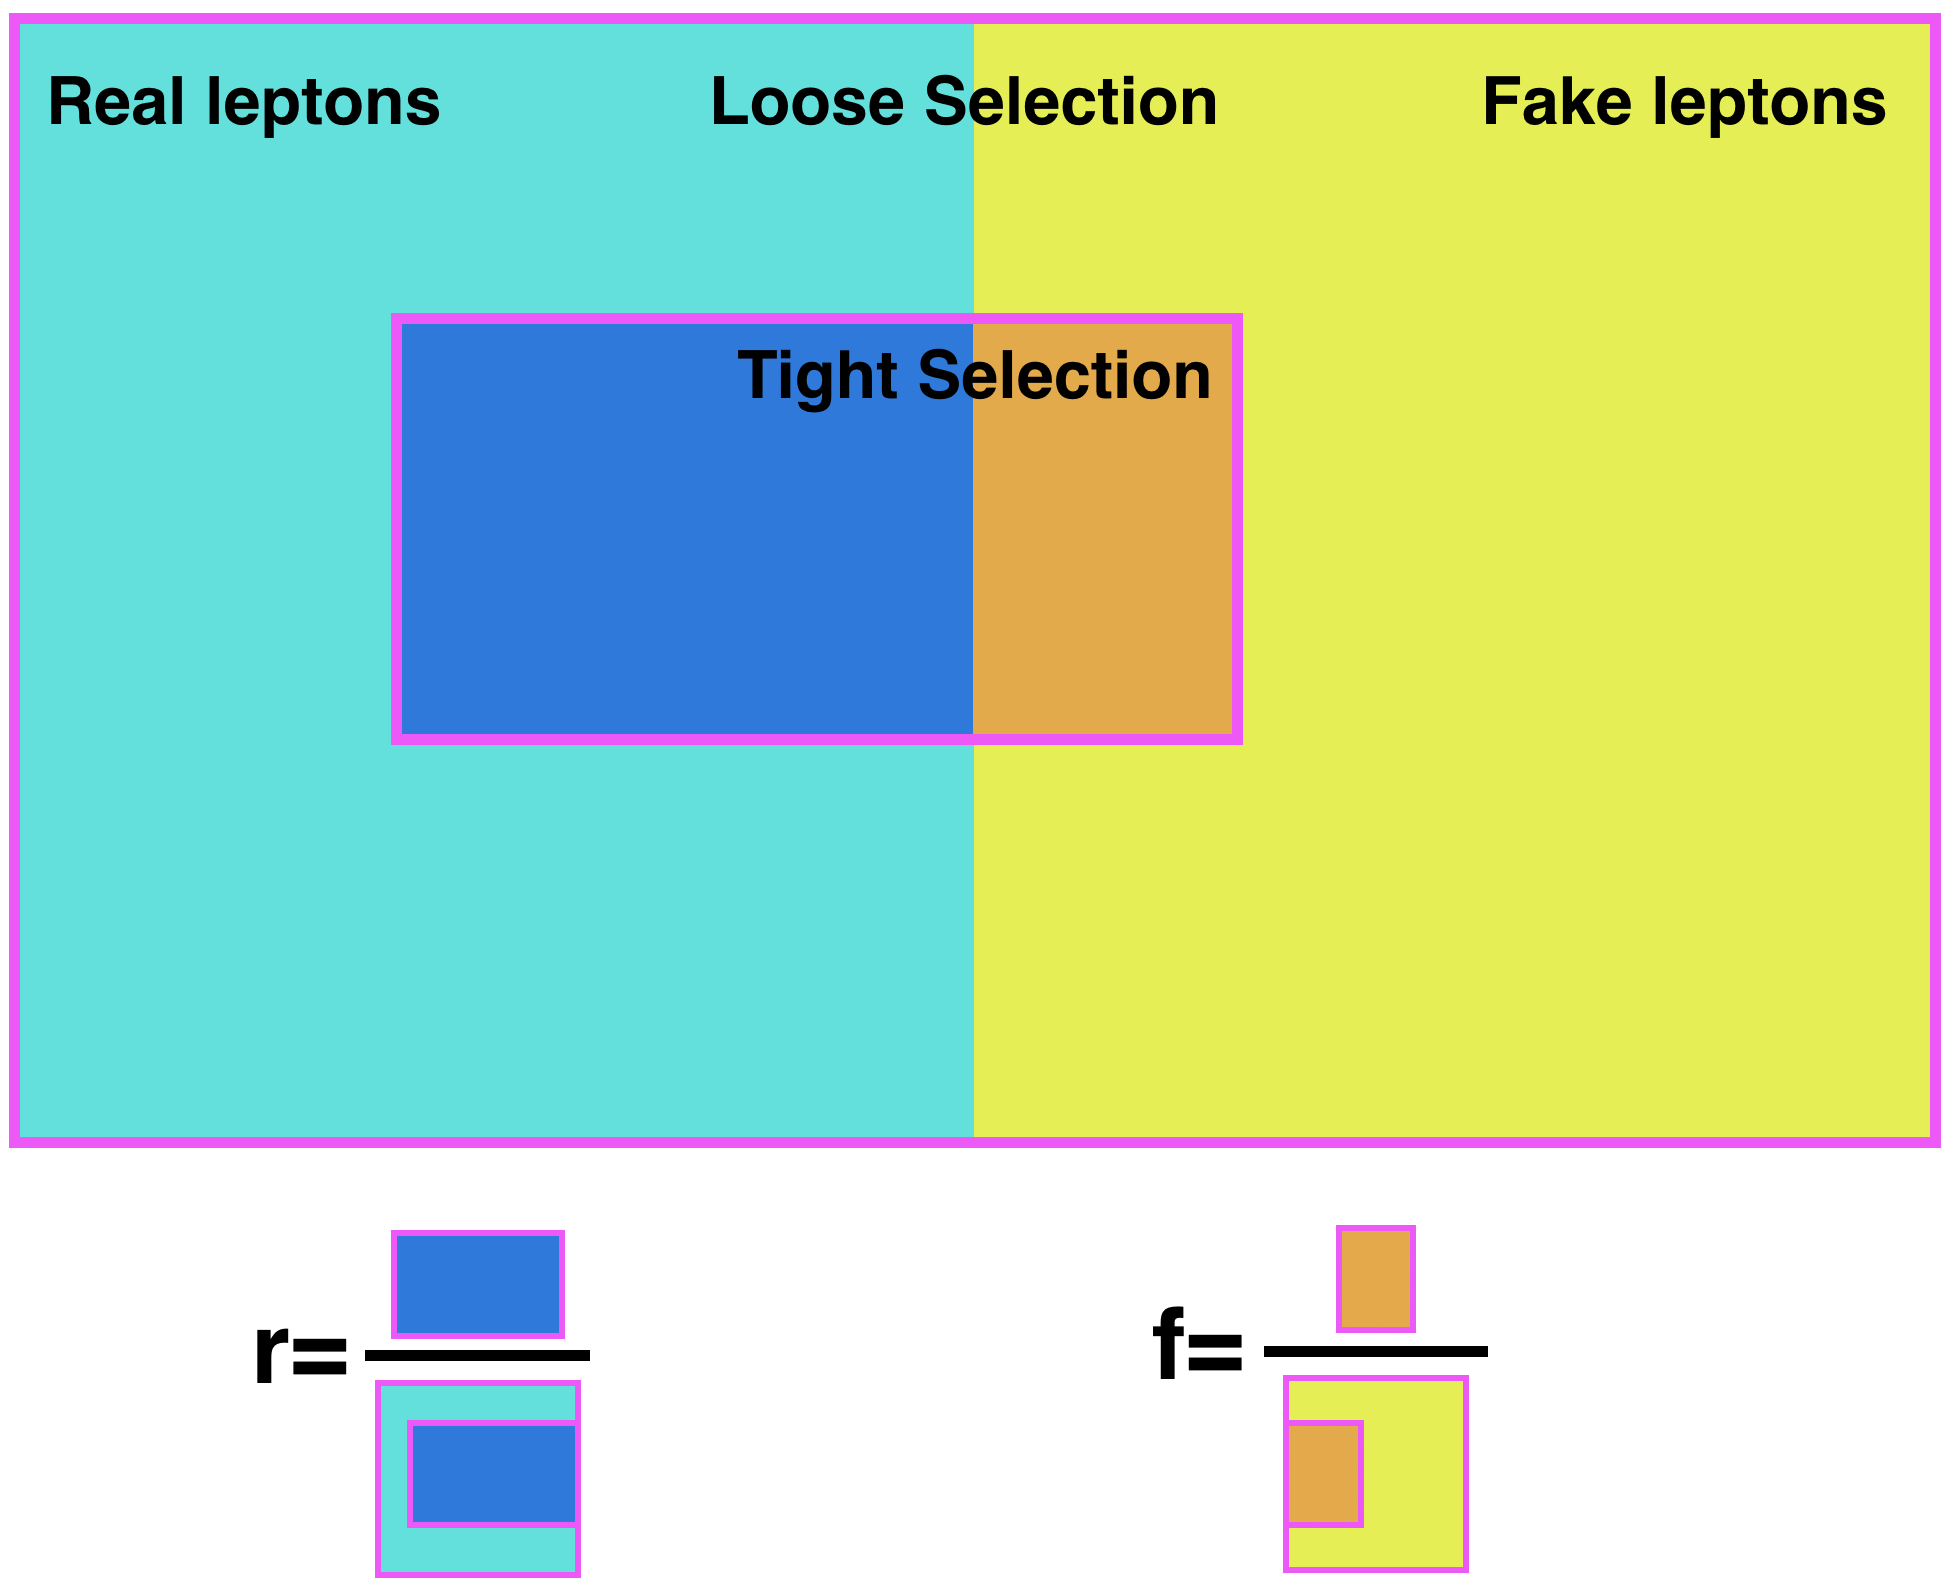
\includegraphics[width=0.8\textwidth]{figures/Part3/Nonprompt/matrix}
 \end{tabular}
 \caption{Illustration of the \emph{prompt} efficiency $r$ and the \emph{nonprompt} efficiency $f$. The \emph{loose} selection is typically a subset of the \emph{tight} selection, which guarantees both $r$ and $f$ to be greater than 0 and smaller 1.}
 \label{fig:Matrix_Method}
 \end{center}
\end{figure}

In a simplified scenario with only one lepton in the final state, the \emph{prompt} efficiency $r$ measures the probability of \emph{prompt} leptons passing \emph{tight} selection. It is treated as an observable that can be obtained through measurement,

\begin{equation}
r=\frac{n_P^{T}}{n_P^{T}+n_P^{\overline{T}}},
 \label{eq:real_rate}
\end{equation}
in which $n_P^{T}$/$n_P^{\overline{T}}$ denotes the number of events with a \emph{prompt} lepton that is \emph{tight}/\emph{not tight}.

Similarly, \emph{nonprompt} efficiency $f$ can be expressed as,

\begin{equation}
f=\frac{n_{N}^{T}}{n_{N}^{T}+n_{N}^{\overline{T}}},
 \label{eq:fake_rate}
\end{equation}
in which $n_{N}^{T}$/$n_{N}^{\overline{T}}$ denotes the number of events with a \emph{nonprompt} lepton that is \emph{tight}/\emph{not tight}.

The measurement of $r/f$ is often performed in dedicated control regions, where high purity of \emph{prompt}/\emph{nonprompt} leptons is expected. These regions are referred to as the \ac{MR}. It is assumed that $r/f$ is a universal property of \emph{prompt}/\emph{nonprompt} leptons that is independent of physics processes. Therefore, $r/f$ extracted from \ac{MR} can be used to estimate the contamination of \emph{nonprompt} leptons in a different region (e.g. \ac{SR}) even though these two regions are orthogonal to each other.

In this simplified scenario, the total number of events in the region of interest (e.g. \ac{SR}/\ac{VR}) with a \emph{tight}/\emph{not tight} lepton can be expressed in a system of equations,

\begin{equation}
\begin{split}
N^{T}&=N_{P}^{T}+N_{N}^{T}\\
N^{\overline{T}}&=N_{P}^{\overline{T}}+N_{N}^{\overline{T}},
\end{split}
\end{equation}

in which the capital letter ``$N$'' is used to indicate that these numbers are referring to events in a region that is different from \ac{MR}. $N_{P}^{\overline{T}}$/$N_{N}^{\overline{T}}$ can be expressed in terms of $r/f$ and $N_{P}^{T}$/$N_{N}^{T}$ according to Equation \ref{eq:real_rate}/\ref{eq:fake_rate} and the assumption that r/f remains the same across different regions,

\begin{equation}
\begin{split}
N^{T}&=r\frac{N_{P}^{T}}{r}+f\frac{N_{N}^{T}}{f}\\
N^{\overline{T}}&=(1-r)\frac{N_{P}^{T}}{r}+(1-f)\frac{N_{N}^{T}}{f}.
\end{split}
\label{eq:sys_eq}
\end{equation}

Equation~\ref{eq:sys_eq} can also be expressed in the form of a matrix,

\begin{equation}
 \begin{pmatrix}
 N^{T}\\
 N^{\overline{T}}
 \end{pmatrix}=\begin{pmatrix}
r&f\\
1-r&1-f
 \end{pmatrix}\begin{pmatrix}
 N_{P}^{T}/r\\
 N_{N}^{T}/f
 \end{pmatrix}.
 \label{eq:matrix}
 \end{equation}
 
Regions that correspond to the two numbers that appear in the right-hand side vector of Equation~\ref{eq:matrix} are referred to as the ``\acp{AR}'', which can be constructed using experimental data. The estimation of \emph{nonprompt} background, denoted by $N_{N}^T$, can be obtained by a simple matrix inversion. 
%%%%%%%%%%%%%%%%%%%%%%%%%%%%%%%%%%%%%%%%%%%%%%%%%%%%%%%%%%%%
%%%%%%%%%%%%%%%%%%%%%%%%%%%%%%%%%%%%%%%%%%%%%%%%%%%%%%%%%%%%

\section{Generialization and Implementation of the Matrix Method}
\label{sec:MR}

The description in the previous section deals with a scenario where only one lepton is studied. This analysis uses a generalized version of the \mm, where all three \emph{tight} leptons are considered to be possibly \emph{nonprompt}. Equation~\ref{eq:matrix} is generalized as,

\begin{equation}
\hspace{-3.7em}
 \resizebox{1.2\linewidth}{!}{%
 $
 \begin{pmatrix}
 N^{TTT}\\\\
 N^{TT\overline{T}}\\\\
 N^{T\overline{T}T}\\\\
 N^{T\overline{T}\overline{T}}\\\\
 N^{\overline{T}TT}\\\\
 N^{\overline{T}T\overline{T}}\\\\
 N^{\overline{T}\overline{T}T}\\\\
 N^{\overline{T}\overline{T}\overline{T}}
 \end{pmatrix}=\begin{pmatrix}
r_1r_2r_3&r_1r_2f_3&r_1f_2r_3&r_1f_2f_3&f_1r_2r_3&f_1r_2f_3&f_1f_2r_3&f_1f_2f_3\\\\
r_1r_2(1-r_3)&r_1r_2(1-f_3)&r_1f_2(1-r_3)&r_1f_2(1-f_3)&f_1r_2(1-r_3)&f_1r_2(1-f_3)&f_1f_2(1-r_3)&f_1f_2(1-f_3)\\\\
r_1(1-r_2)r_3&r_1(1-r_2)f_3&r_1(1-f_2)r_3&r_1(1-f_2)f_3&f_1(1-r_2)r_3&f_1(1-r_2)f_3&f_1(1-f_2)r_3&f_1(1-f_2)f_3\\\\
r_1(1-r_2)(1-r_3)&r_1(1-r_2)(1-f_3)&r_1(1-f_2)(1-r_3)&r_1(1-f_2)(1-f_3)&f_1(1-r_2)(1-r_3)&f_1(1-r_2)(1-f_3)&f_1(1-f_2)(1-r_3)&f_1(1-f_2)(1-f_3)\\\\
(1-r_1)r_2r_3&(1-r_1)r_2f_3&(1-r_1)f_2r_3&(1-r_1)f_2f_3&(1-f_1)r_2r_3&(1-f_1)r_2f_3&(1-f_1)f_2r_3&(1-f_1)f_2f_3\\\\
(1-r_1)r_2(1-r_3)&(1-r_1)r_2(1-f_3)&(1-r_1)f_2(1-r_3)&(1-r_1)f_2(1-f_30&(1-f_1)r_2(1-r_3)&(1-f_1)r_2(1-f_3)&(1-f_1)f_2(1-r_3)&(1-f_1)f_2(1-f_3)\\\\
(1-r_1)(1-r_2)r_3&(1-r_1)(1-r_2)f_3&(1-r_1)(1-f_2)r_3&(1-r_1)(1-f_2)f_3&(1-f_1)(1-r_2)r_3&(1-f_1)(1-r_2)f_3&(1-f_1)(1-f_2)r_3&(1-f_1)(1-f_2)f_3\\\\
(1-r_1)(1-r_2)(1-r_3)&(1-r_1)(1-r_2)(1-f_3)&(1-r_1)(1-f_2)(1-r_3)&(1-r_1)(1-f_2)(1-f_3)&(1-f_1)(1-r_2)(1-r_3)&(1-f_1)(1-r_2)(1-f_3)&(1-f_1)(1-f_2)(1-r_3)&(1-f_1)(1-f_2)(1-f_3)
 \end{pmatrix}\begin{pmatrix}
 N_{PPP}^{TTT}/r_1r_2r_3\\\\
 N_{PPN}^{TTT}/r_1r_2f_3\\\\
 N_{PNP}^{TTT}/r_1f_2r_3\\\\  
 N_{PNN}^{TTT}/r_1f_2f_3\\\\
 N_{NPP}^{TTT}/f_1r_2r_3\\\\
 N_{NPN}^{TTT}/f_1r_2f_3\\\\
 N_{NNP}^{TTT}/f_1f_2r_3\\\\
 N_{NNN}^{TTT}/f_1f_2f_3
 \end{pmatrix}.
 $}
 \label{eq:matrix_method3}
 \end{equation}
 
Except for the first number, all other numbers that appear in the right-hand side vector correspond to events with at least one \emph{nonprompt} lepton that passes \emph{tight} selection criteria. Therefore, the overall \emph{nonprompt} background is expresses as,
 
\begin{equation}
N_{Nonprompt}^{TTT} = N_{PPN}^{TTT} + N_{PNP}^{TTT} + N_{PNN}^{TTT} + N_{NPP}^{TTT} + N_{NPN}^{TTT} + N_{NNP}^{TTT} + N_{NNN}^{TTT},
\end{equation}
 
which can be obtained by first constructing 8 \acp{AR} to form the lefthand side vector. Secondly, the 8 $\times$ 8 matrix is constructed and inverted. Lastly, the righthand side vector can be obtained by multiplying the lefthand side vector by the inverted matrix.

Only two \acp{PD} ``SingleElectron'' and ``SingleMuon'' are used in the construction of \ac{MR} in 2016 and 2017 while ``SingleElectron'' is replaced with ``EGamma'' in 2018. In addition to \acp{PD}, the measurements of $r$/$f$ also utilize the $\ttbar$ sample and all \ac{MC} samples listed under the ``\emph{prompt} background'' category in Table~\ref{tab:MCsample}. Depending on the flavor of the leading lepton in \ac{MC}, events are selected with either a single-electron or a single-muon trigger, which is summarized in Table~\ref{tab:RandF_trigger}. Data events are selected with the same \ac{HLT} triggers as well but events in ``SingleMuon'' (``SingleElectron'' or ``EGamma'') \ac{PD} are only accepted if the leading lepton is a muon (electron).

\begin{table}[th]
\sffamily
\centering
\caption{Summary of the \ac{HLT} triggers used in the measurement of $r$ and $f$. These are unprescaled single-lepton triggers with the lowest $\pt$ threshold. The threshold of the electron trigger is higher in the 2017 and 2017 datasets due to increased instantaneous luminosity in those two years.}
\begin{tabular}{llllll}
\toprule
Channel  & Path    & Dataset & 2016 & 2017 & 2018 \\ \midrule
\multirow{2}{*}{Electron} & HLT\_Ele27\_WPTight\_Gsf & Data \& MC & \checkmark & - & - \\ 
      & HLT\_Ele35\_WPTight\_Gsf & Data \& MC & - & \checkmark & \checkmark \\ \hline
\multirow{1}{*}{Muon} & HLT\_IsoMu27 & Data \& MC & \checkmark & \checkmark & \checkmark \\ \bottomrule
\end{tabular}
\label{tab:RandF_trigger}
\end{table}

Both $r$ and $f$ are parameterized in bins of lepton $\pt$, $|\eta|$, and jet multiplicity. The bin range is optimized to retain sufficient statistics for each bin:

\begin{itemize}
\item Electron $\pt$ bin range: \{20.0, 24.6, 28.8, 33.0, 37.2, 41.4, 46.1, 52.1, 59.3, 68.3, 82.7, 110.6\} GeV,
\item Muon $\pt$ bin range: \{20.0, 23.8, 27.7, 31.3, 35.0, 38.9, 42.8, 45.6, 50.7, 59.5, 72.9, 94.3\} GeV,
\item $|\eta|$ bin range: \{0, 0.8, 1.6, 2.4\},
\item Jet multiplicity: \{0 jets, $\geq$ 1 jet\}.
\end{itemize}

The jet multiplicity bin is a proxy for variation in the composition of physics processes. In addition to requiring at least one jet, the \ac{MR} corresponds to the second jet multiplicity bin requires no more than one b-tagged jet as this is also required in the \ac{SR}.

The \emph{nonprompt} efficiency is measured in same-sign dilepton regions, in which the leading lepton in $\pt$, used as a \emph{tag}, is required to be matched with trigger objects within $\mathrm{\Delta}R~<$ 0.2. The sub-leading lepton is required to pass the \emph{loose} selection and is taken as the \emph{probe}. Events that have two same-sign electrons with an invariant mass between 76 and 106 GeV are removed from \ac{MR} to suppress the backgrounds that originate from charge misidentification. No such requirement has been introduced to the muon \ac{MR} due to its negligible rate of charge misidentification.

The contribution from \emph{prompt} backgrounds, estimated from \ac{MC} simulation, is subtracted from the data. A representative composition of backgrounds in \ac{MR} is shown in Figure~\ref{fig:MRexample}. 

\begin{figure}[tbh!]
 \begin{center}
 \begin{tabular}{cc}
 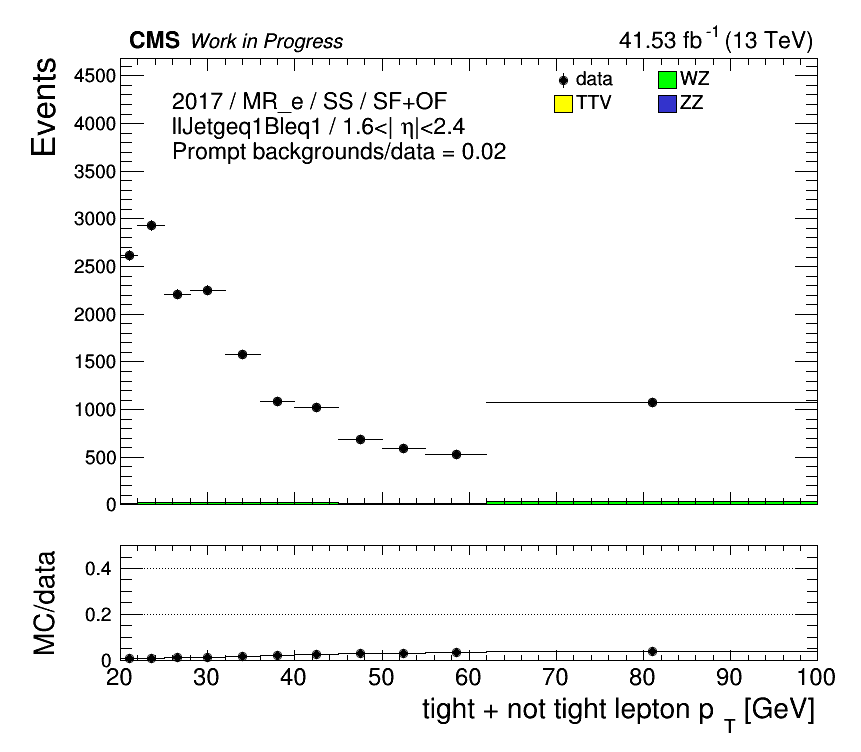
\includegraphics[width=0.45\textwidth]{figures/Part3/Nonprompt/MR/FlepPt}&
 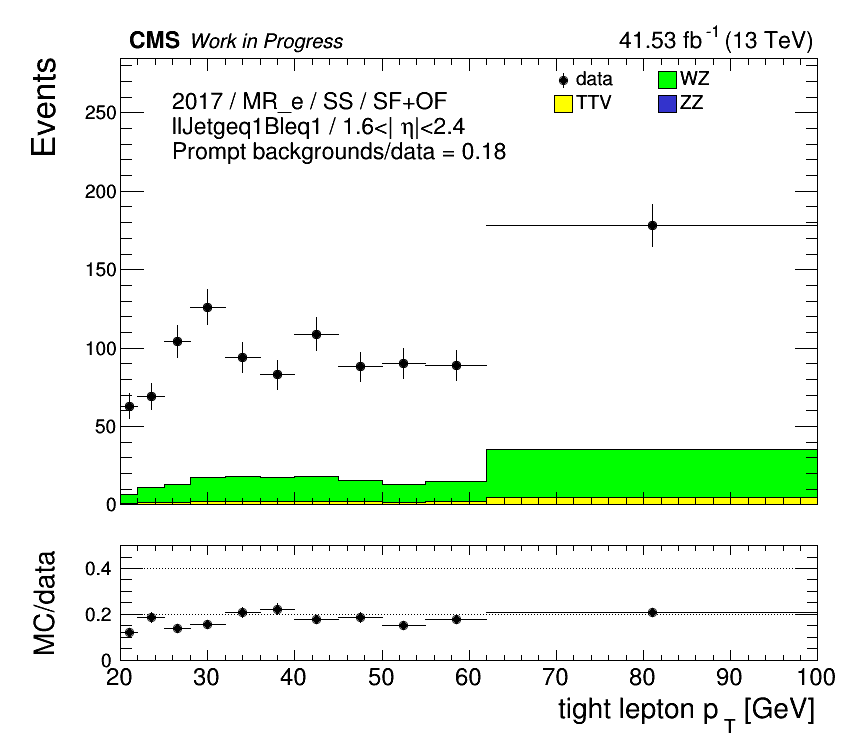
\includegraphics[width=0.45\textwidth]{figures/Part3/Nonprompt/MR/TlepPt} \\
 \end{tabular}
 \caption{Distribution of lepton $\pt$ in a representative electron \emph{nonprompt} efficiency \ac{MR}. In this particular example, both ee and $\upmu$e flavor composites are considered. At least one jet and at most one b-tagged jet are required (the second jet multiplicity bin). \emph{Probe} electron is required to have $1.6<|\eta|<2.4$ (the third $\eta$ bin). Contamination from \emph{prompt} backgrounds are estimated with \ac{MC} simulation, and are shown as histograms. The data are shown as filled points. From left to right: \emph{loose} (i.e. \emph{tight + not tight}) electron $\pt$, \emph{tight} electron $\pt$.}
 \label{fig:MRexample}
 \end{center}
\end{figure}

The \emph{nonprompt} efficiency $f$ is calculated as:

\begin{equation}
f=\frac{n_{data}^{tag+tight}-n_{MC(prompt)}^{tag+tight}}{n_{data}^{tag+loose}-n_{MC(prompt)}^{tag+loose}},
\label{eq:f_eq}
\end{equation}  

where the numerator is selected with one \emph{tag} and one \emph{tight} lepton while the denominator is selected with one \emph{tag} and one \emph{loose} lepton. The selection criteria for \emph{tag}, \emph{loose}, and \emph{tight} lepton is summarised in Table~\ref{tab:MR}.

\begin{table}[th]
\sffamily
\centering
\caption{Summary of the lepton selections needed for the measurement of $r$ and $f$. Please note: (i) the minimum $\pt$ cut for \emph{tag} electron in the 2016 dataset is reduced to 30 GeV to adjust for the trigger threshold, and (ii) the \emph{tight} selection here is the same as the \emph{tight} lepton selection described in \autoref{sec:Leptons}.}
\begin{tabular}{ccccc}
\toprule
Lepton  &Selection  & \emph{loose} & \emph{tag} & \emph{tight}$^{\textsf{ii}}$\\ \midrule
\multirow{4}{*}{Electron} & $\pt$ & $>$ 20 GeV & $>$ 38 GeV$^{\textsf{i}}$ & $>$ 20 GeV \\  
   & $I_{\textsf{mini}}^{\textsf{rel}}$ & $<$0.4 & $<$0.1 & $<$0.12 \\
   & \TOP  & $>$-0.9  & $>$0.95 & $>$0.9 \\ 
   & Match with trigger objects  & - & \checkmark & - \\ \midrule
\multirow{5}{*}{Muon} & $\pt$ & $>$ 20 GeV & $>$ 30 GeV & $>$ 20 GeV \\
   & $I_{\textsf{mini}}^{\textsf{rel}}$ & $<$0.4 & $<$0.1 & $<$0.12 \\
   & Cut-based ID & - & Medium WP & Medium WP \\
   & \TOP  & $>$0.5 & $>$0.9 & $>$0.9 \\ 
   & Match with trigger objects  & - & \checkmark & - \\ \bottomrule
\end{tabular}
\label{tab:looseandtight}
\end{table}

\begin{figure}[tbh!]
 \begin{center}
 \begin{tabular}{c}
 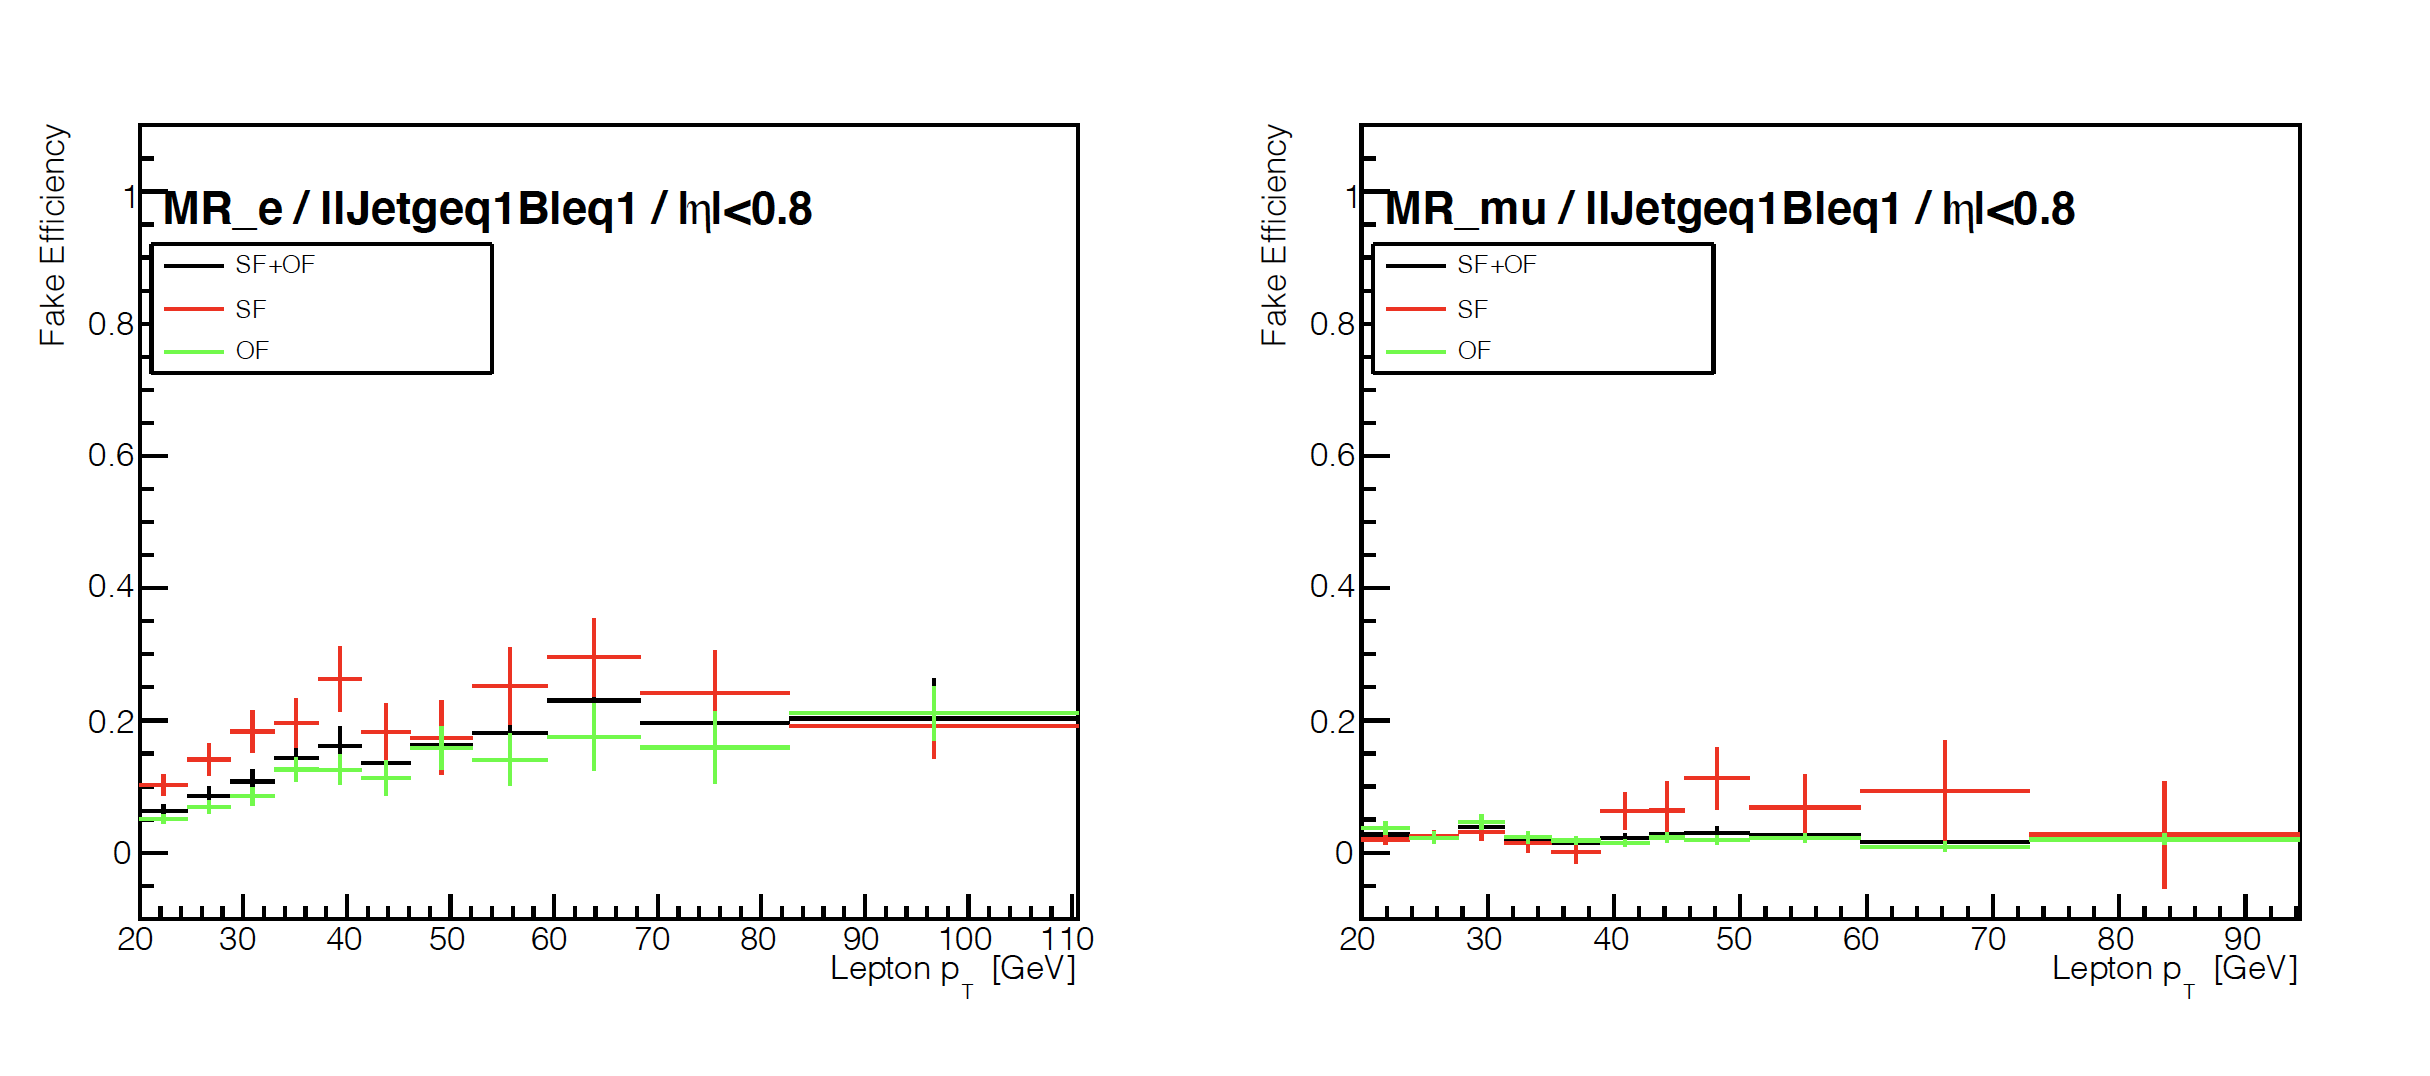
\includegraphics[width=0.85\textwidth]{figures/Part3/Nonprompt/MR/fake_eff}
 \end{tabular}
 \caption{Representative \emph{nonprompt} electron efficiency measured in data events. From left to right: electron $f$, muon $f$. Events with a same-flavor lepton pair are shown in red points while events selected with a different-flavor lepton pair are shown in green points. Events with a same-flavor or different-flavor lepton pair are shown in black points. These plots correspond to the first $|\eta|$ bin ($|\eta|<$0.8) and the second jet multiplicity bin. Events selected Error bars displayed in these plots include statistical uncertainty only. }
 \label{fig:fake_eff}
 \end{center}
\end{figure}

The measured \emph{nonprompt} efficiency $f$ exhibits a dependency on flavor composition, as is shown in Figure~\ref{fig:fake_eff}. This dependency is treated as a source of the systematic uncertainties of the \emph{nonprompt} estimation and is further discussed in \autoref{sec:NonUnc}.

The \emph{prompt} efficiency $r$ is measured in simulated $\ttbar$ events in opposite-sign dilepton regions. The same lepton selection listed in Table~\ref{tab:looseandtight} is used to perform the \emph{Tag-and-Probe}. The leading lepton in $\pt$ is used as a \emph{tag} while the oppositely charged sub-leading lepton is taken as a \emph{probe}. The variation of $r$ between different flavor compositions is negligible, as is shown in Figure~\ref{fig:real_eff}. Therefore, only e$\upmu$ events are used to measure \emph{prompt} efficiency in order to minimize the contamination of \emph{nonprompt} leptons.

\begin{figure}[tbh!]
 \begin{center}
 \begin{tabular}{c}
 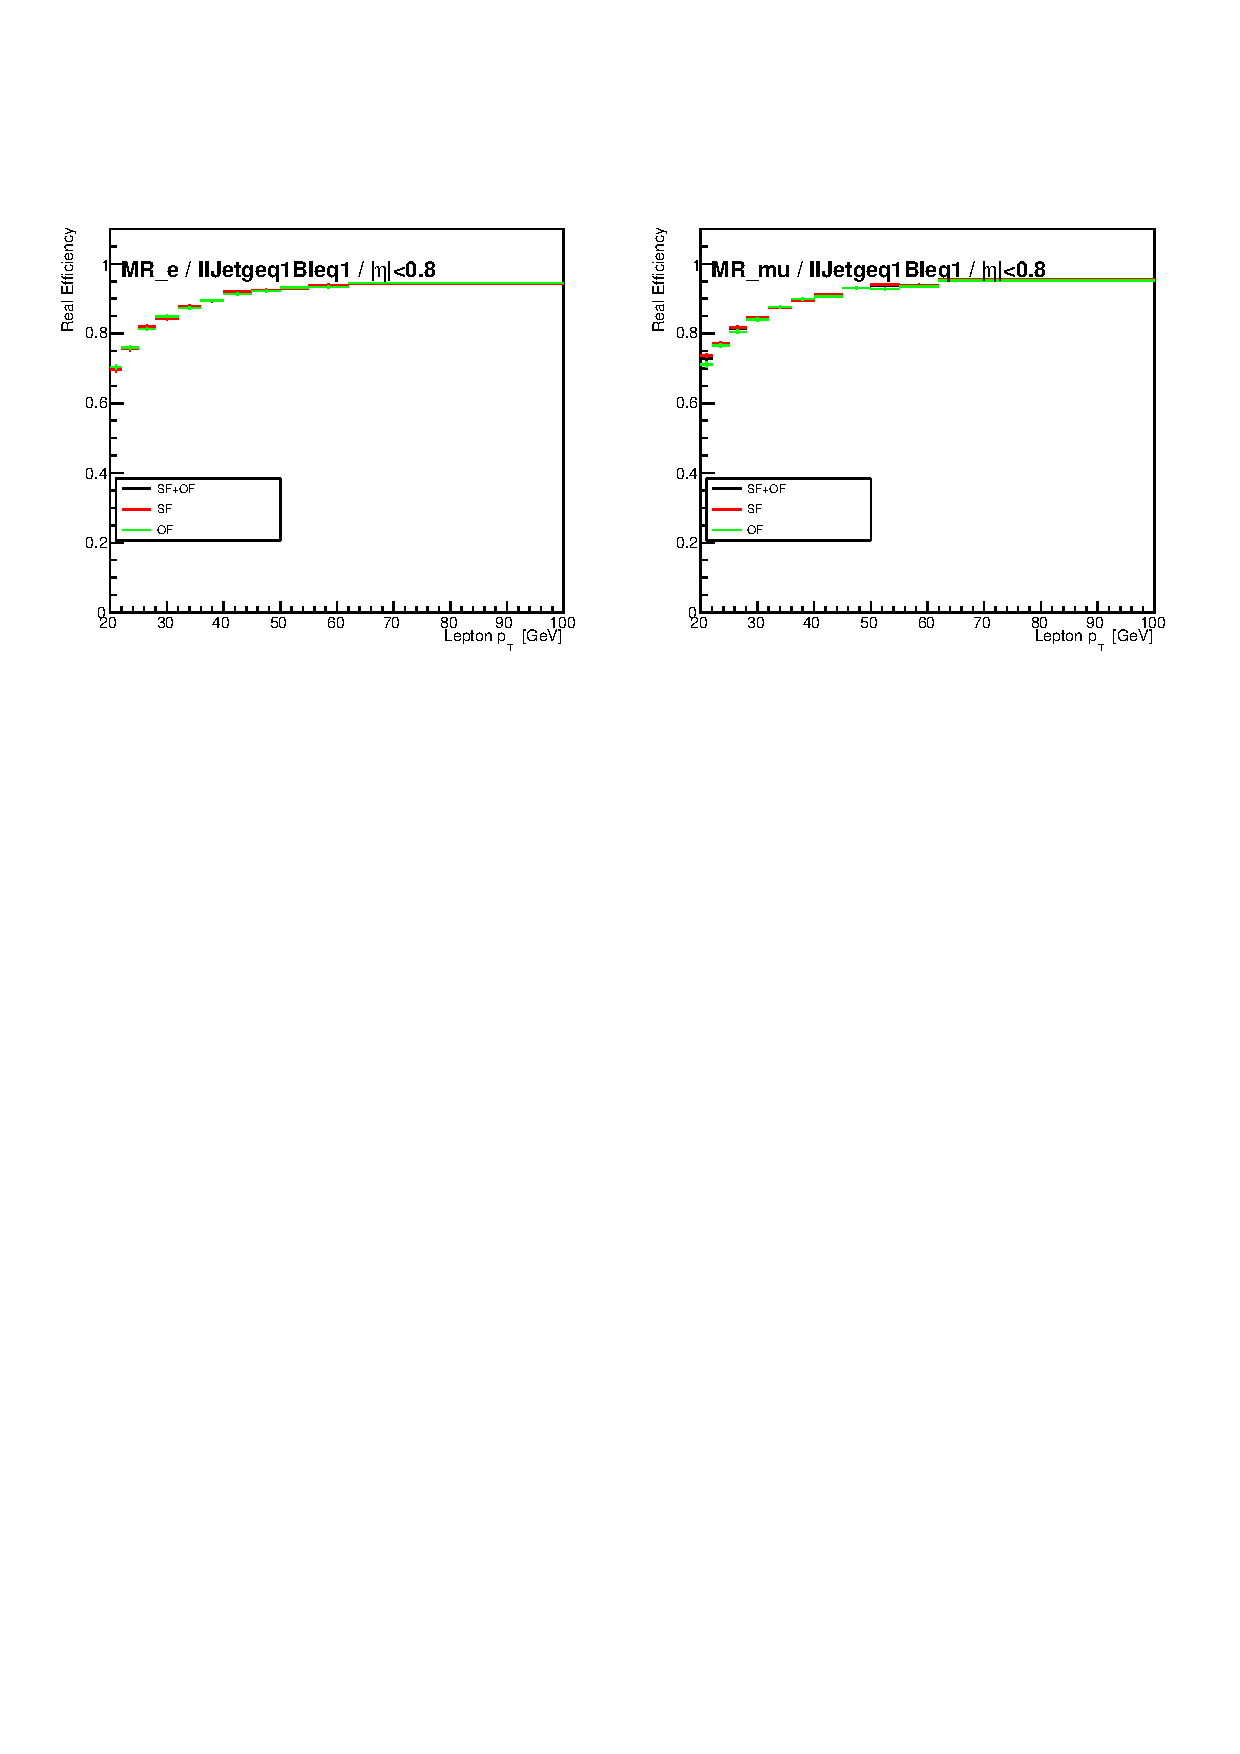
\includegraphics[width=0.85\textwidth]{figures/Part3/Nonprompt/MR/real_eff}
 \end{tabular}
 \caption{Representative \emph{prompt} efficiency measured in simulated $\ttbar$ events. From left to right: electron $r$, muon $r$. Events with a same-flavor lepton pair are shown in red points while events selected with a different-flavor lepton pair are shown in green points. Events with a same-flavor or different-flavor lepton pair are shown in black points. These plots correspond to the first $|\eta|$ bin ($|\eta|<$0.8) and the second jet multiplicity bin. Error bars displayed in these plots include statistical uncertainty only. }
 \label{fig:real_eff}
 \end{center}
\end{figure}

The selection criteria for various \acp{MR} is summarised in Table~\ref{tab:MR}.

\begin{table}[th]
\sffamily
\centering
\caption{Summary of the selection criteria applied to the measurement regions of $r$ and $f$. ``OffZ'' means events containing two same-sign electrons with an in variant mass between 76 and 106 GeV are removed. $C_i$ denotes the electric charge of the selected lepton.}
\resizebox{\textwidth}{!}{ 
\begin{tabular}{cccccccc}
\toprule
\multirow{2}{*}{Observable}  & \multirow{2}{*}{jet bin}     & \multirow{2}{*}{\vtop{\hbox{\strut $\#$ of selected}\hbox{\strut~~~leptons}}} &  \multirow{2}{*}{\vtop{\hbox{\strut lepton flavor}\hbox{\strut~composite}}} & \multirow{2}{*}{$|\sum_iC_i|$} & \multirow{2}{*}{OffZ}        & \multirow{2}{*}{njet} & \multirow{2}{*}{nbjet}\\ 
  & & &  & &        &  & \\ \midrule
\multirow{2}{*}{$f$}   & 0 jet        & 2                & any                  & 2            & same-sign ee  & = 0          & = 0  \\  
                  & 1 or more jet & 2                & any                 & 2             & same-sign ee  & $\geq$ 1 & $\leq$ 1\\ \midrule
\multirow{2}{*}{$r$}  & 0 jet        & 2                 & e$\upmu$ only           & 0            & -  & = 0           & = 0   \\  
                 & 1 or more jet & 2                 & e$\upmu$ only           & 0            & -   & $\geq$ 1 & $\leq$ 1 \\ \bottomrule  
\end{tabular}
}
\label{tab:MR}
\end{table}
%%%%%%%%%%%%%%%%%%%%%%%%%%%%%%%%%%%%%%%%%%%%%%%%%%%%%%%%%%%%
%%%%%%%%%%%%%%%%%%%%%%%%%%%%%%%%%%%%%%%%%%%%%%%%%%%%%%%%%%%%

\section{Validation of the Matrix Method}
\label{sec:MMVR}

The performance of the \mm~is validated using three regions that are tangential to the \ac{SR}, referred to as \acp{VR}. In these \acp{VR}, \emph{prompt} backgrounds are estimated using \ac{MC} simulation while \emph{nonprompt} background is estimated with the \mm. A summary of the selections applied to these VRs is given in \autoref{chap:Selection}. 

Distribution of the leading lepton $\eta$ and jet multiplicity are shown in Figure~\ref{fig:VR_matrix}. Good agreement between data and background estimate has been observed in all three \acp{VR}.

\begin{figure}[tbh!]
 \begin{center}
 \begin{tabular}{cc}
 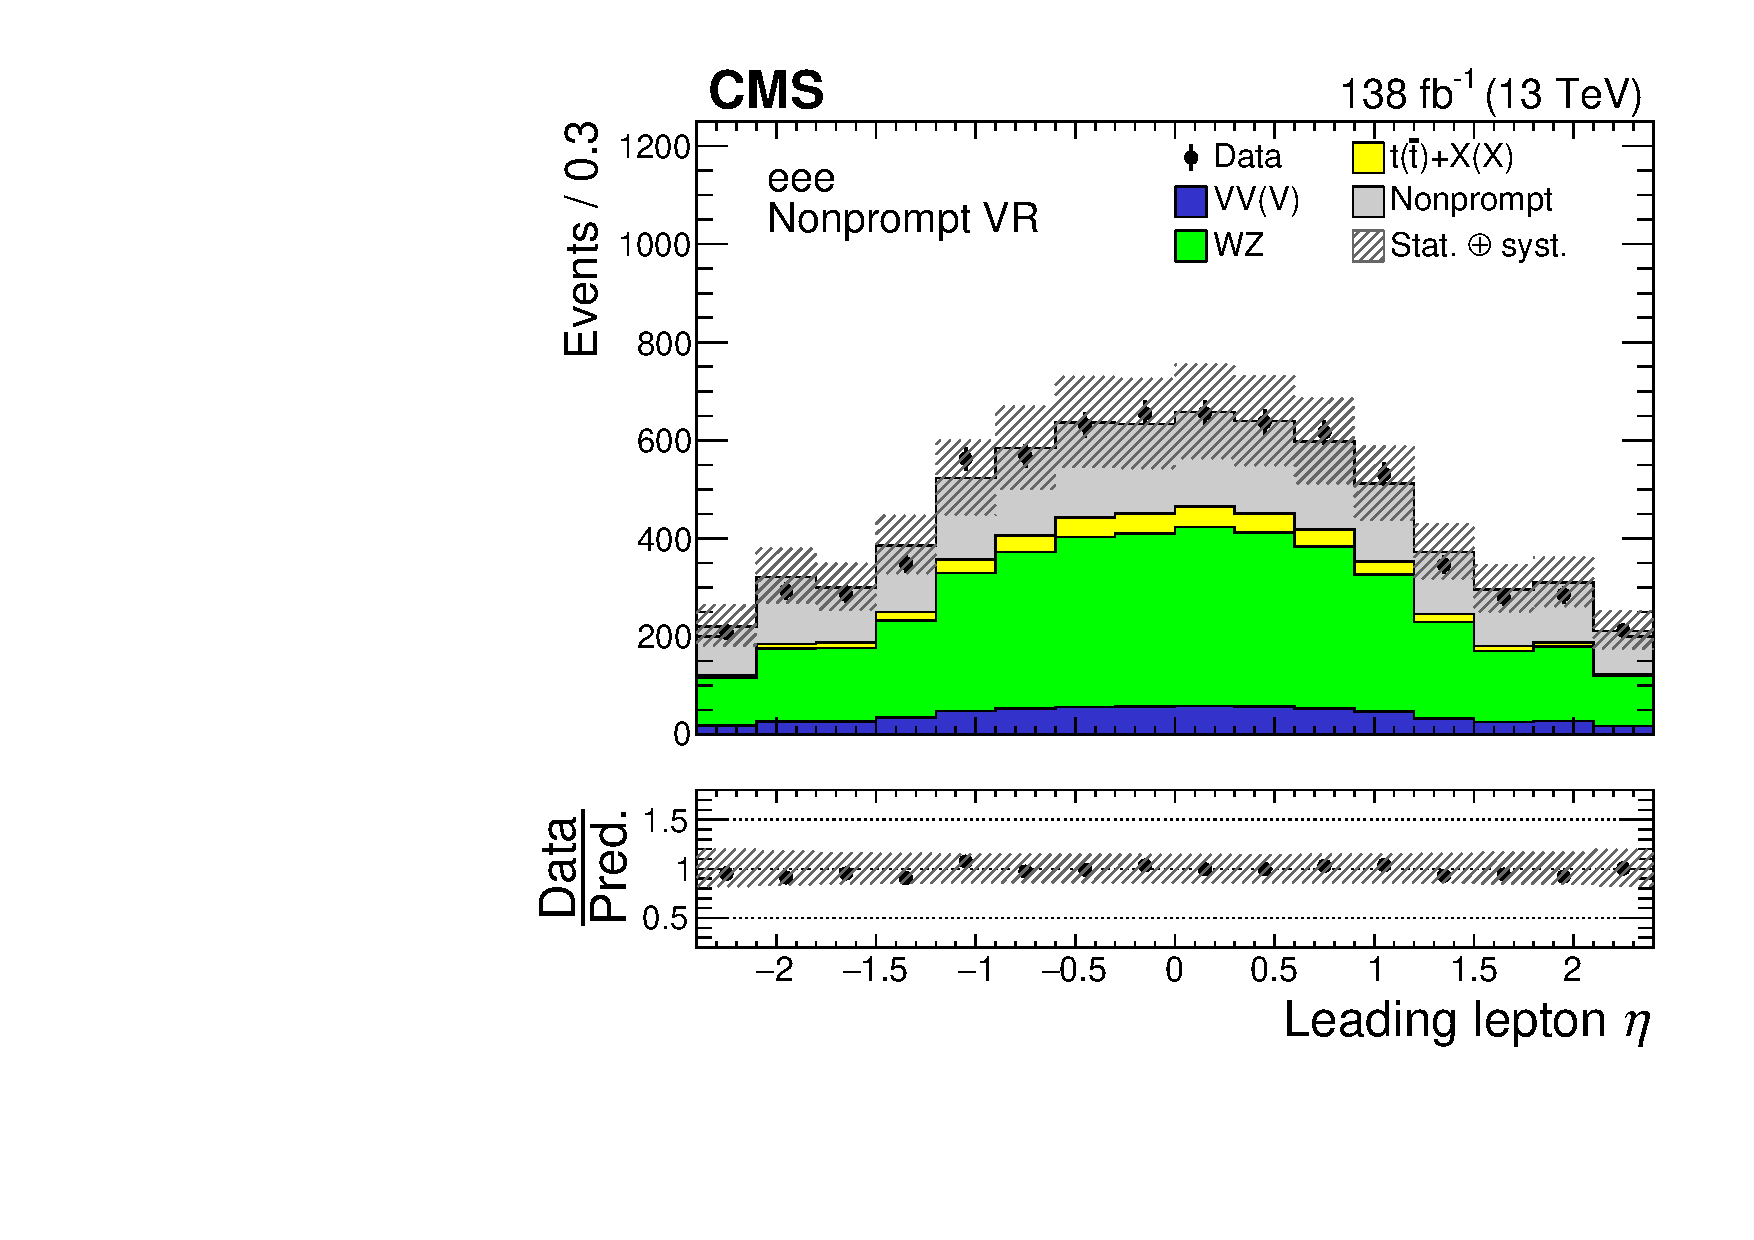
\includegraphics[width=0.45\textwidth]{figures/Part3/Nonprompt/VR/eee/lep1Eta}&
 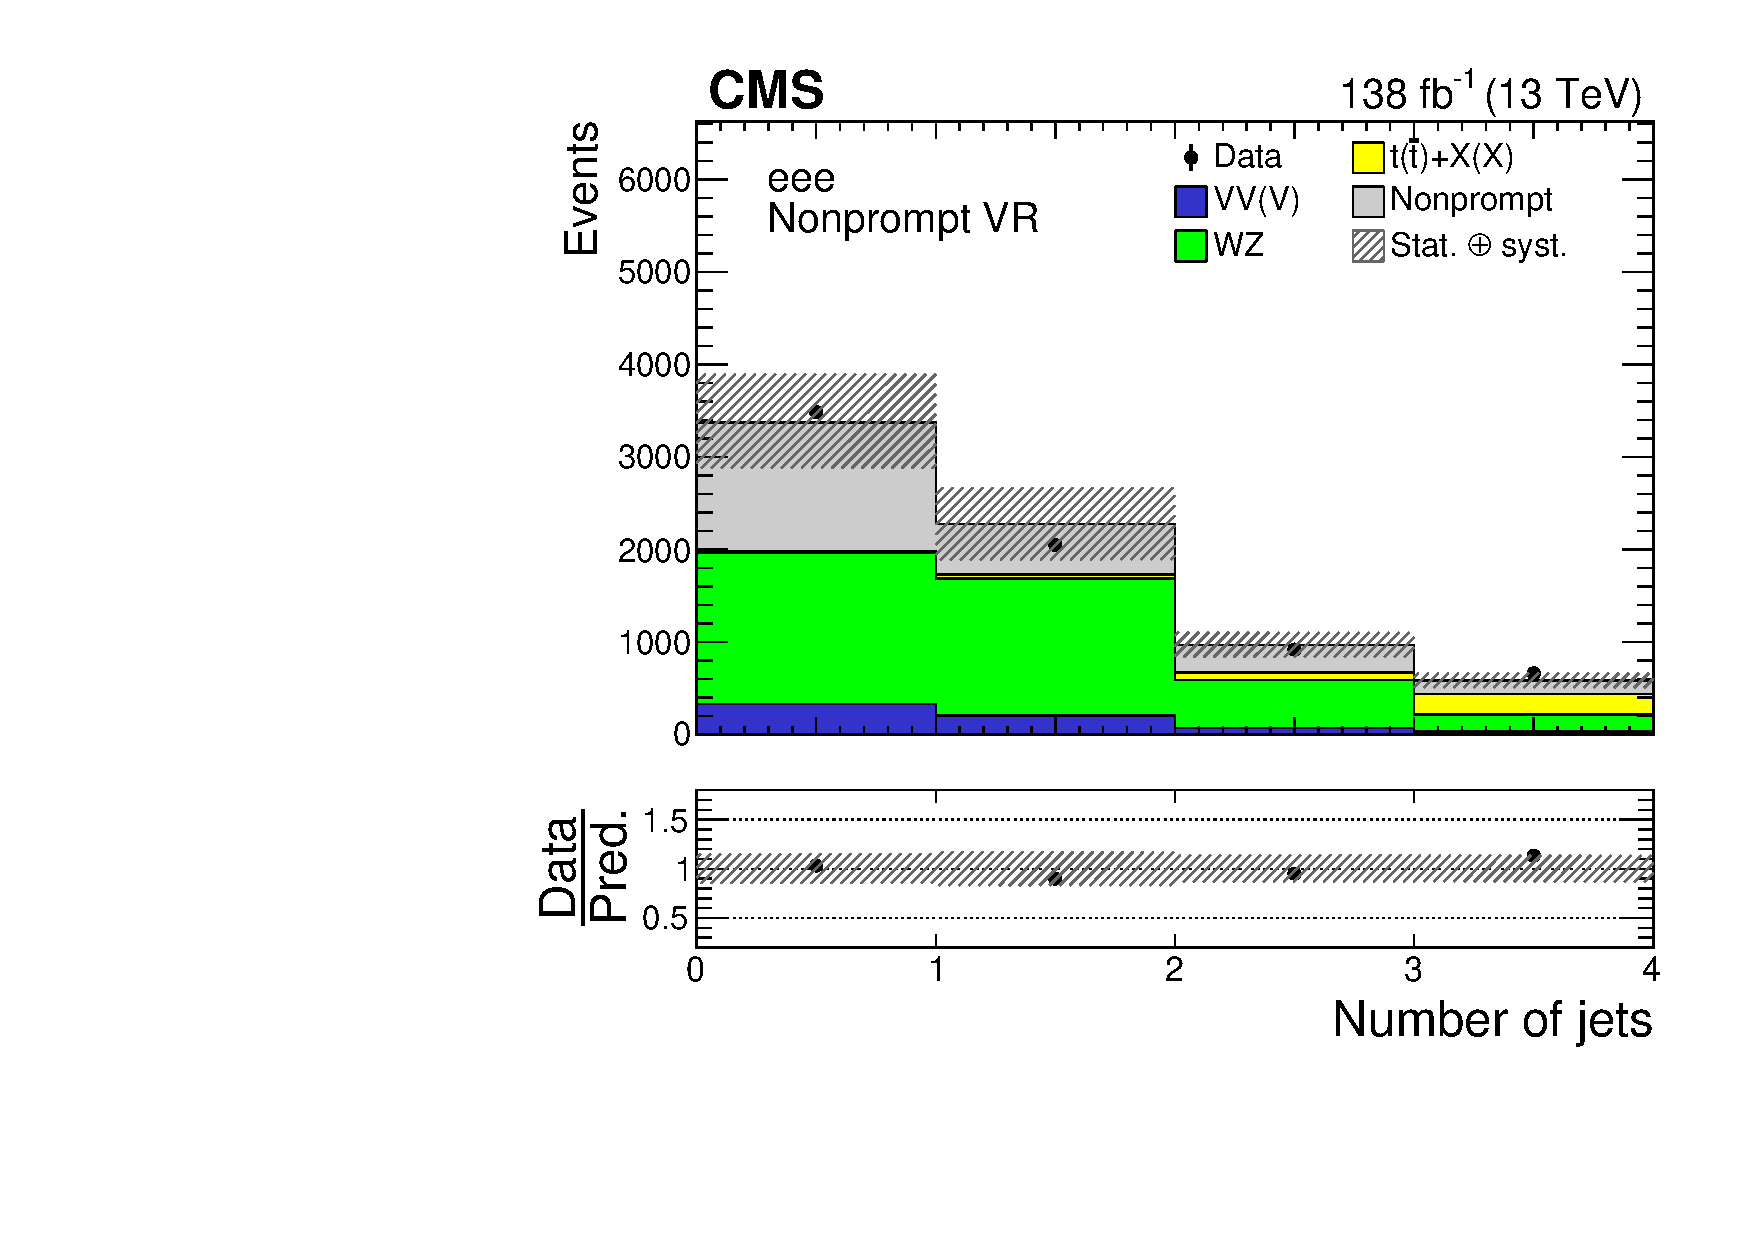
\includegraphics[width=0.45\textwidth]{figures/Part3/Nonprompt/VR/eee/njet} \\
  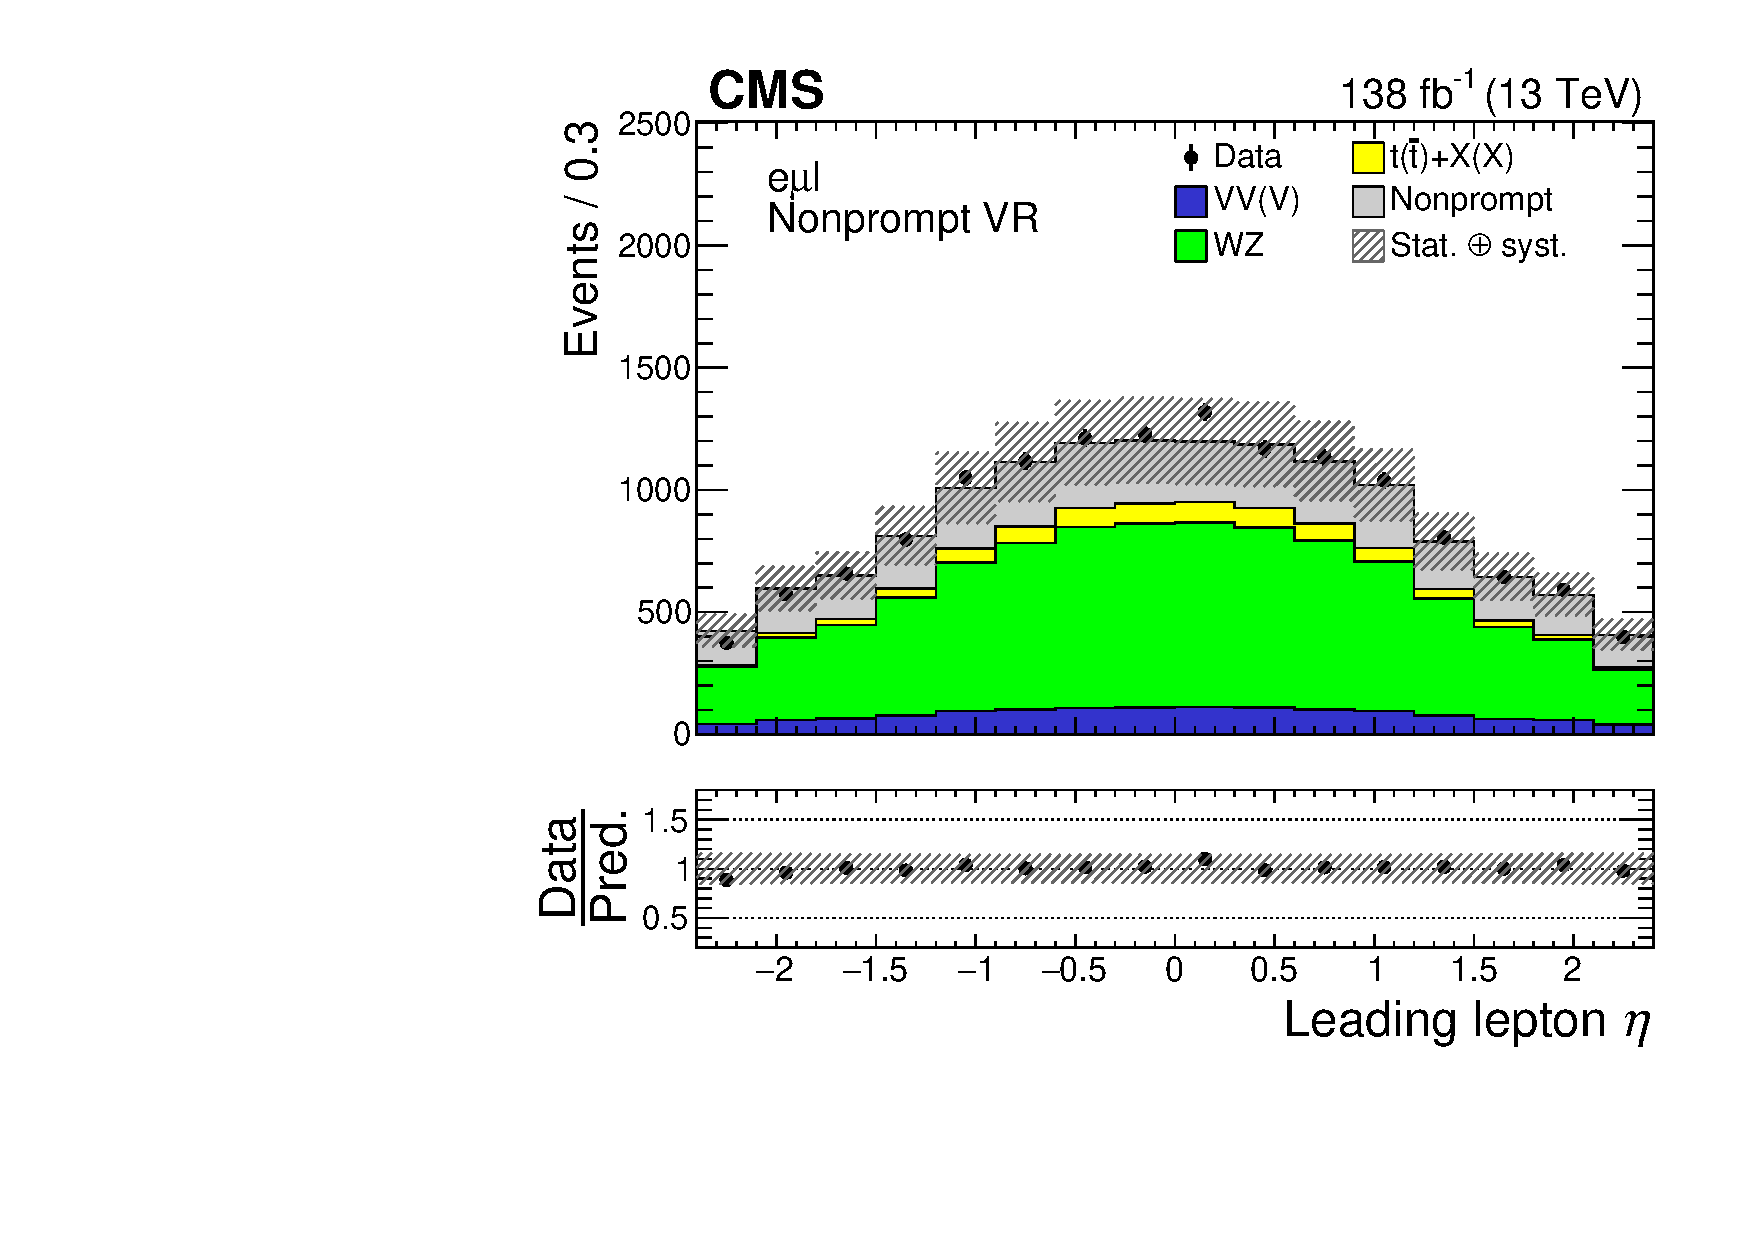
\includegraphics[width=0.45\textwidth]{figures/Part3/Nonprompt/VR/emul/lep1Eta}&
 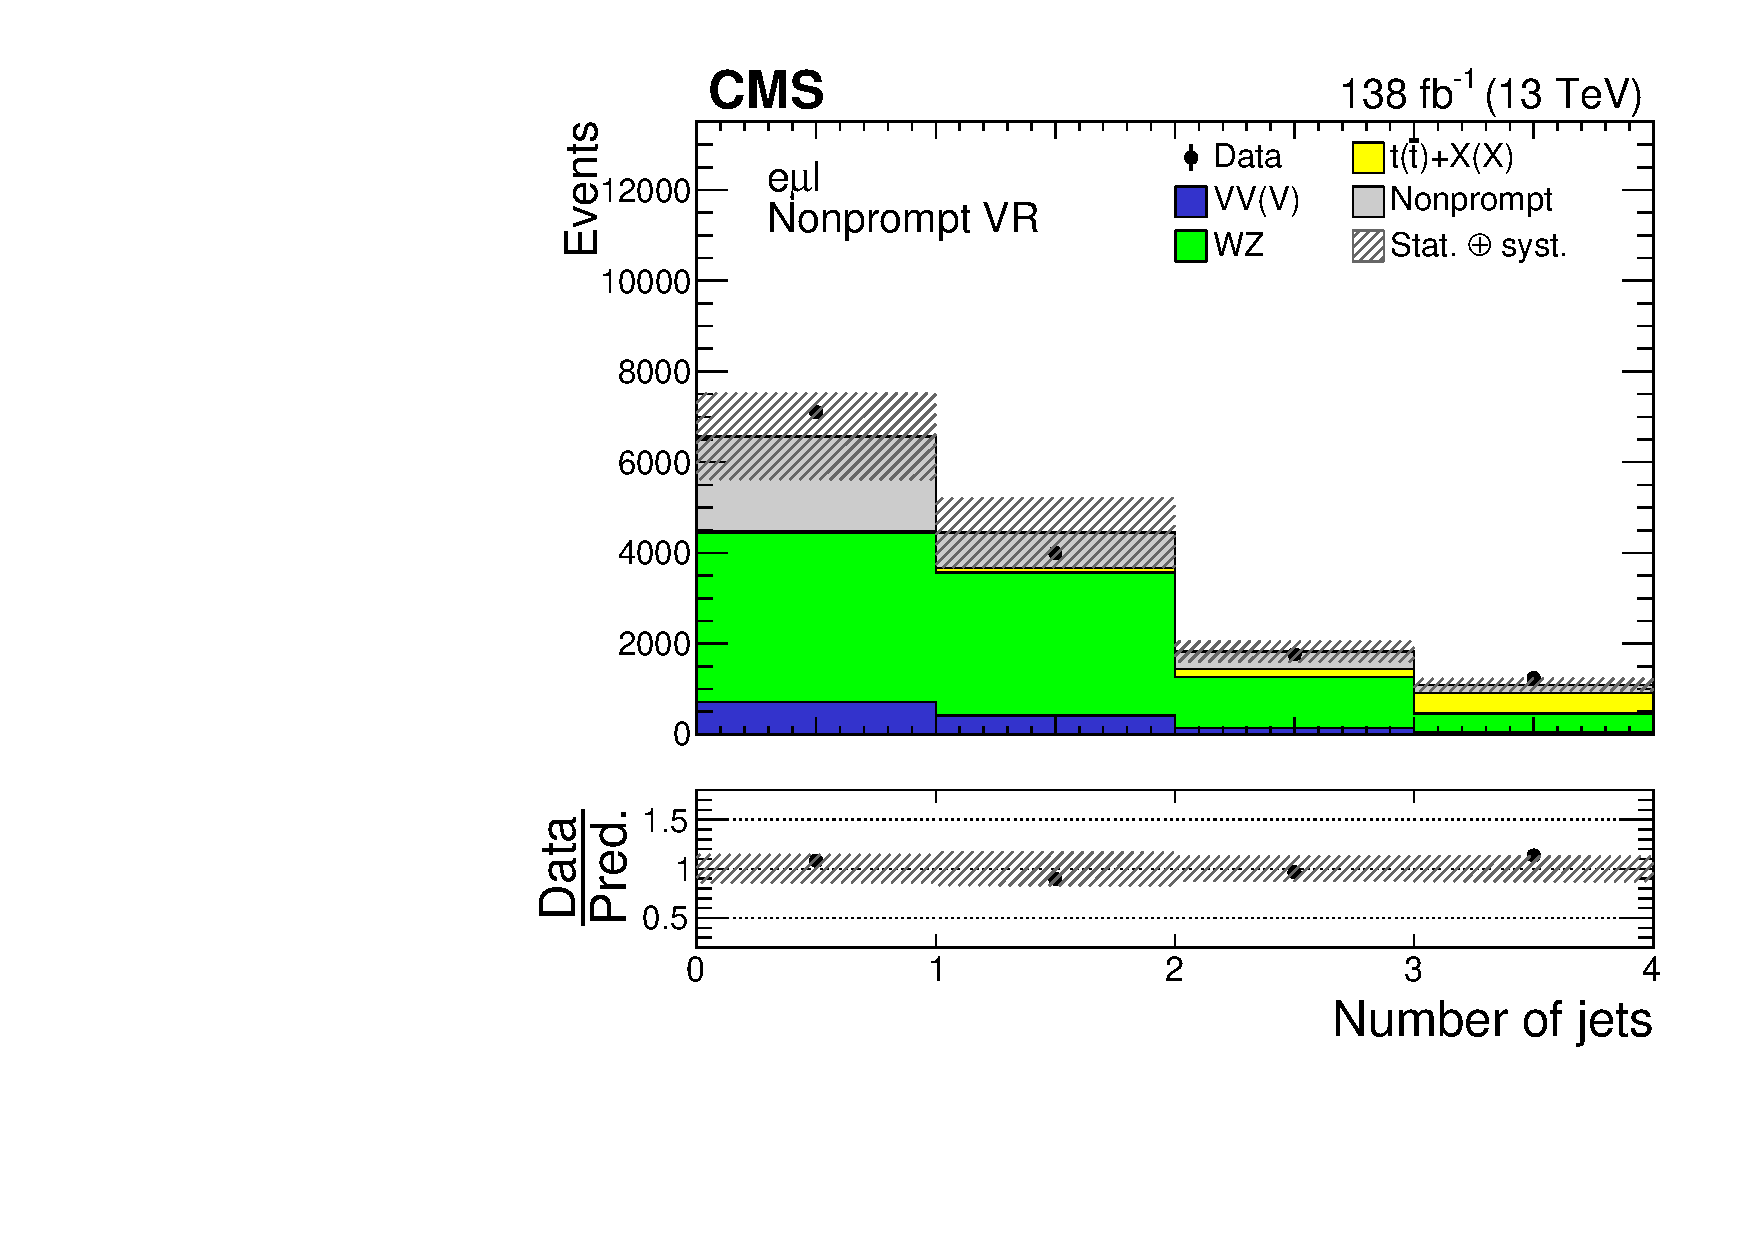
\includegraphics[width=0.45\textwidth]{figures/Part3/Nonprompt/VR/emul/njet} \\
  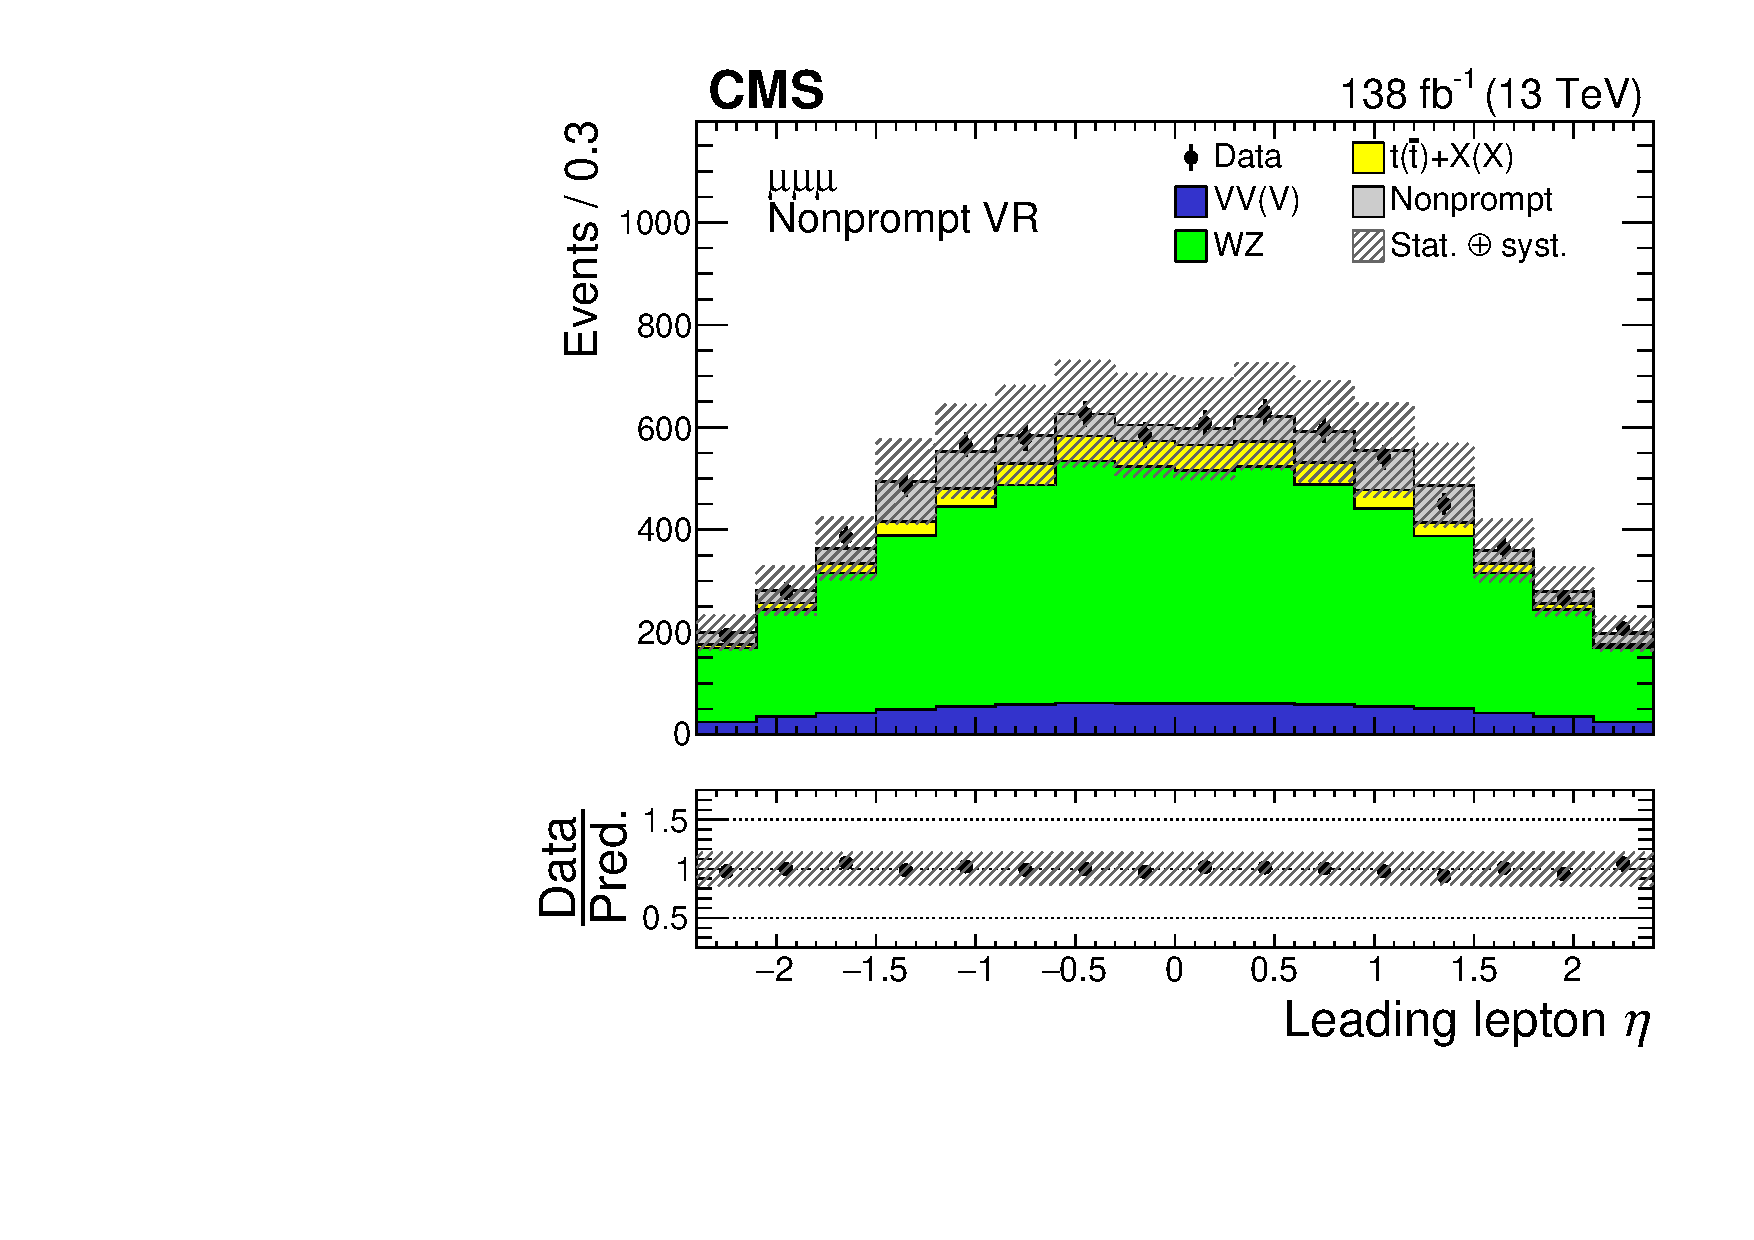
\includegraphics[width=0.45\textwidth]{figures/Part3/Nonprompt/VR/mumumu/lep1Eta}&
 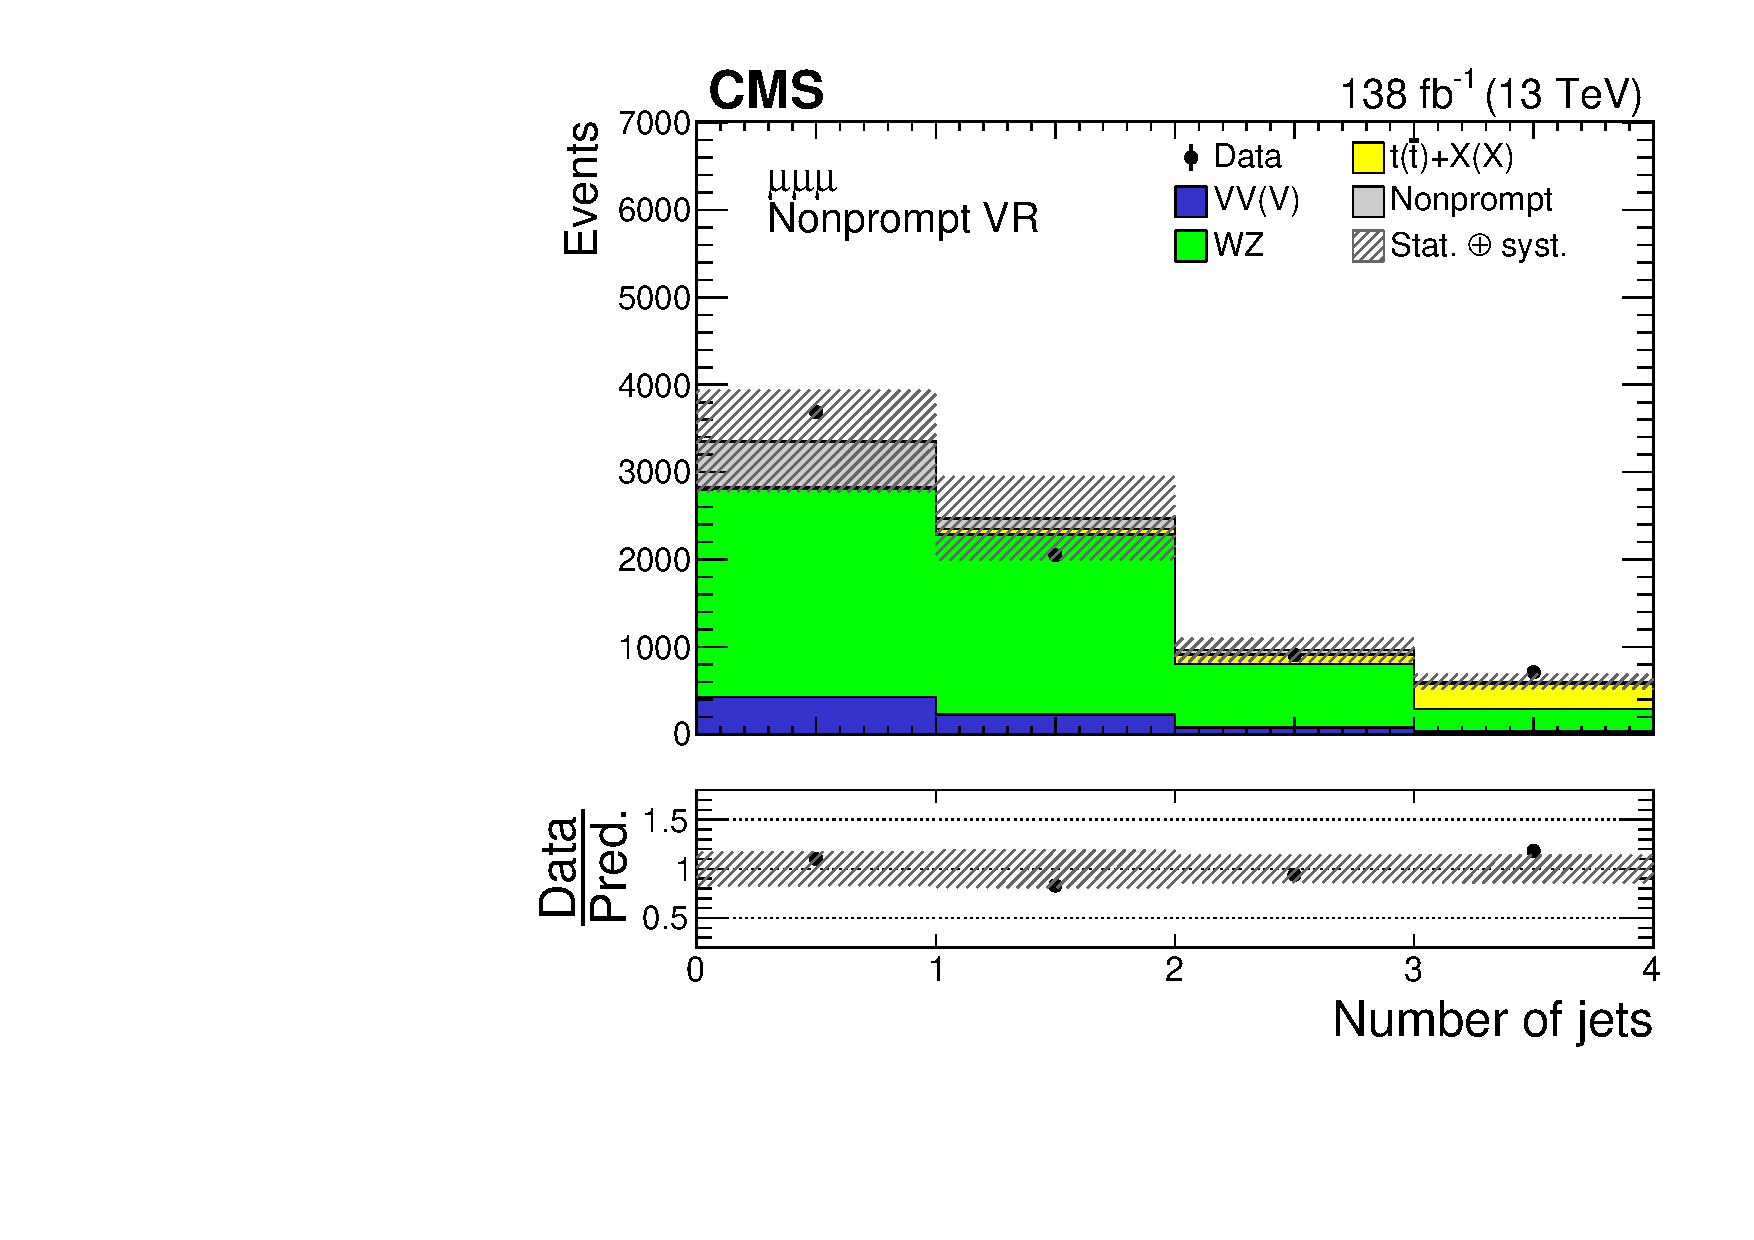
\includegraphics[width=0.45\textwidth]{figures/Part3/Nonprompt/VR/mumumu/njet} \\
 \end{tabular}
 \caption{Distributions of the leading lepton $\eta$ (left column) and the jet multiplicity (right column) in the \emph{nonprompt} \acp{VR}. Events in the eee, $\emul$, and $\mmm$ \emph{nonprompt} \acp{VR} are shown in the upper, middle, and lower row, respectively. The data are shown as filled points and the \ac{SM} background predictions as histograms. The \emph{nonprompt} background is estimated using control samples in data, while other backgrounds are estimated using \ac{MC} simulation. The hatched bands indicate statistical and systematic uncertainties for the \ac{SM} background predictions. The last bin of the right histogram includes the overflow events.}
 \label{fig:VR_matrix}
 \end{center}
\end{figure}
%%%%%%%%%%%%%%%%%%%%%%%%%%%%%%%%%%%%%%%%%%%%%%%%%%%%%%%%%%
%%%%%%%%%%%%%%%%%%%%%%%%%%%%%%%%%%%%%%%%%%%%%%%%%%%%%%%%%%

\section{Nonprompt Estimate in SR}
\label{sec:MMSR}

The \mm~is used to estimate \emph{nonprompt} background in the \ac{SR}. Distributions of the LFV e$\upmu$ mass and the Z boson mass are shown in Figure~\ref{fig:SR_DataDriven_1}. When compared to the background estimate from pure \ac{MC} simulation (Figure~\ref{fig:SR}), the updated background template is smoother with lower statistical uncertainties. 

\begin{figure}[tbh!]
 \begin{center}
 \begin{tabular}{cc}
 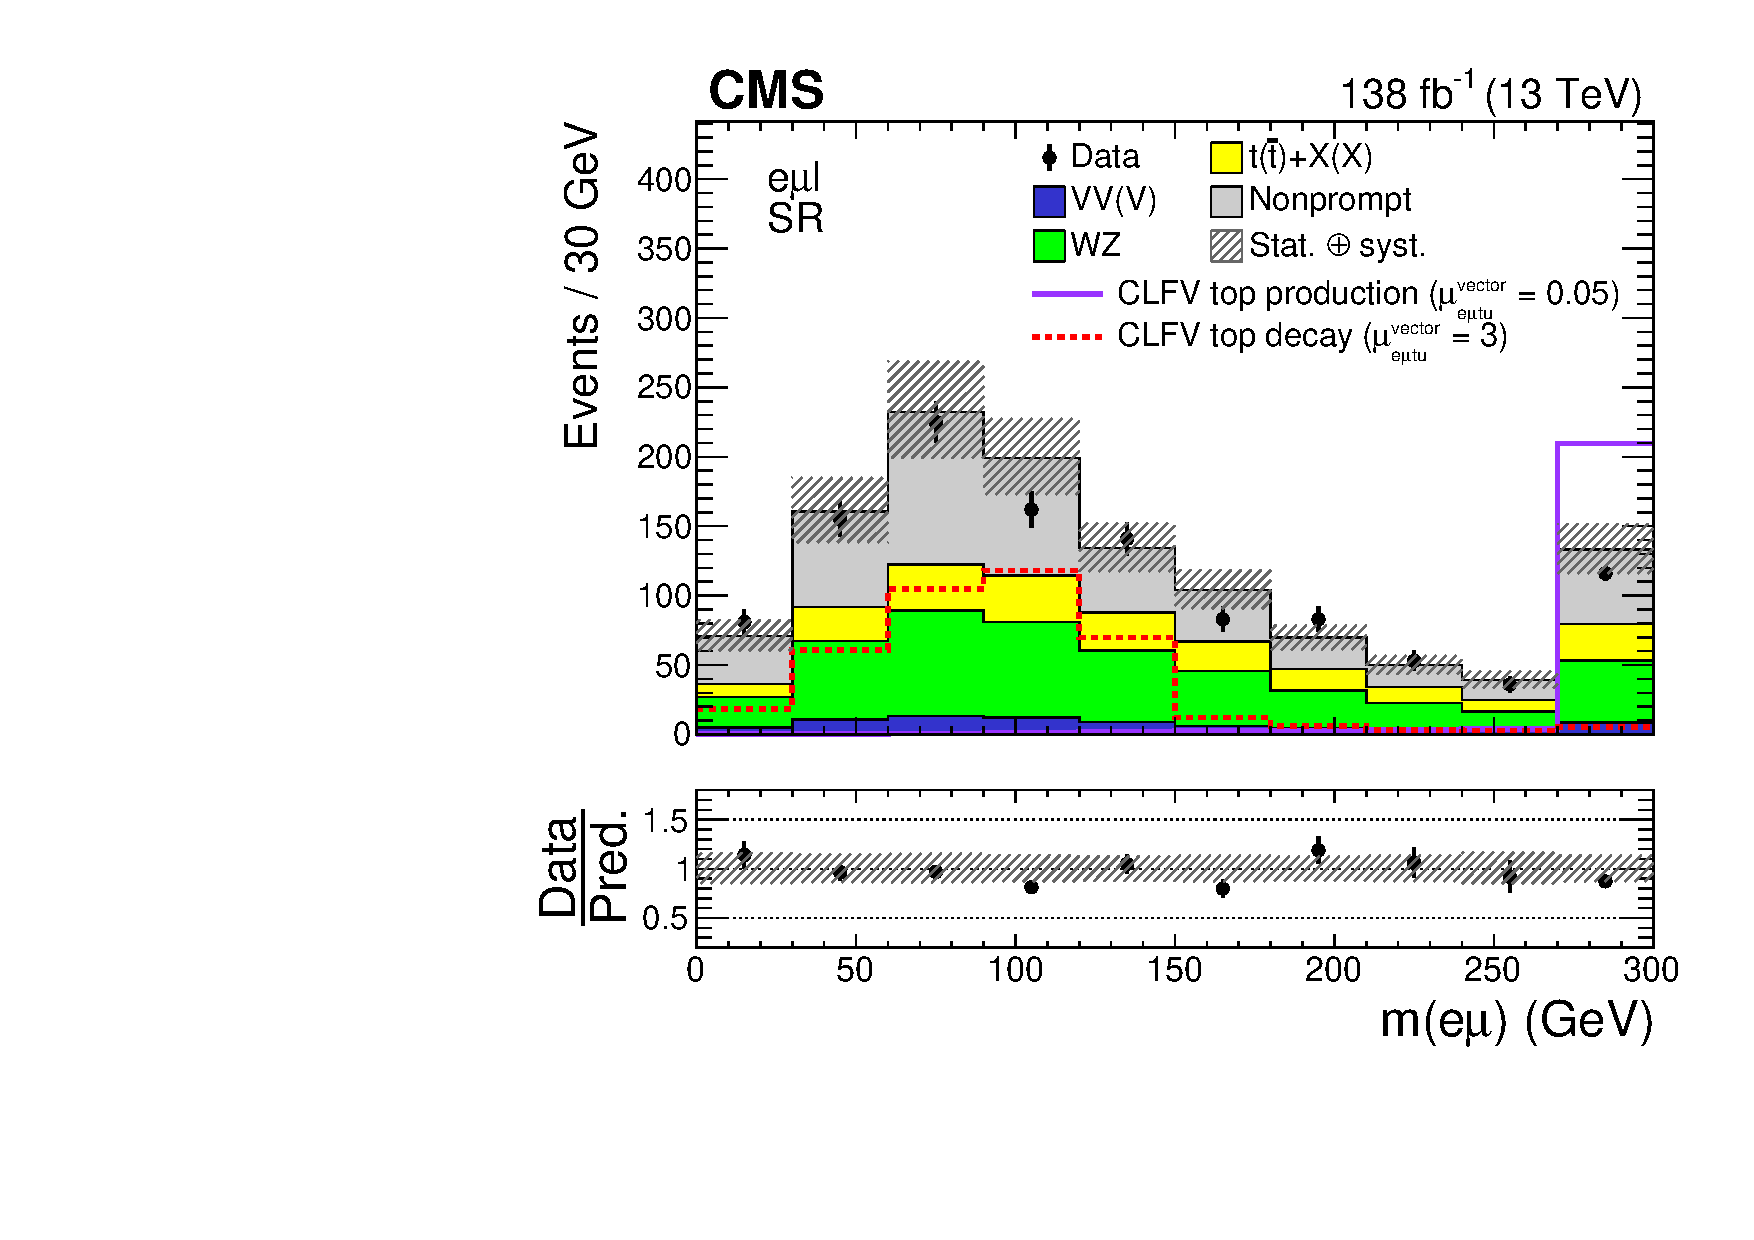
\includegraphics[width=0.45\textwidth]{figures/Part3/Nonprompt/SR/Memu}&
 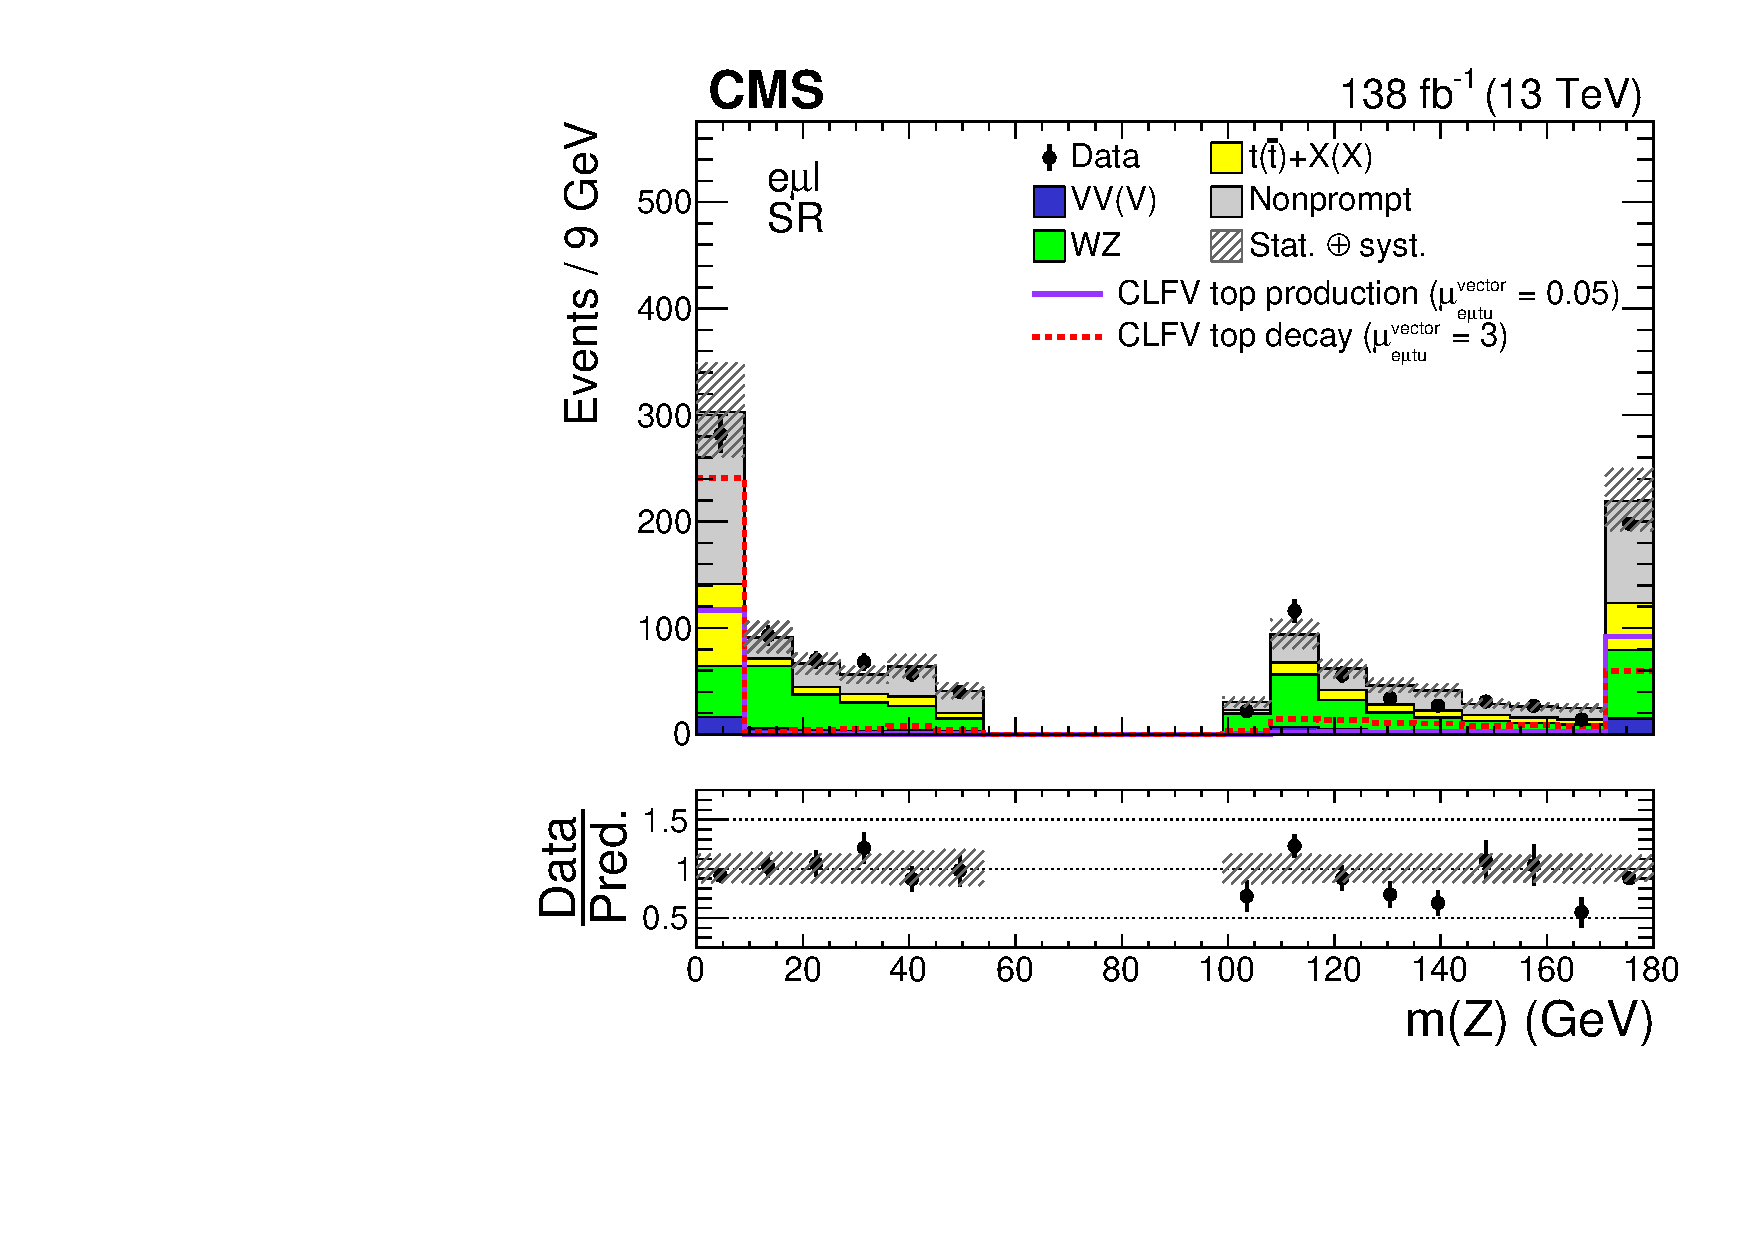
\includegraphics[width=0.45\textwidth]{figures/Part3/Nonprompt/SR/Zmass} \\
 \end{tabular}
 \caption{Distributions of the LFV e$\upmu$ mass (left) and the Z boson mass (right) in \ac{SR}. The data are shown as filled points and the \ac{SM} background predictions as histograms. The \emph{nonprompt} background is estimated using control samples in data, while other backgrounds are estimated using \ac{MC} simulation. The hatched bands indicate statistical and systematic uncertainties for the \ac{SM} background predictions. The normalization of the signal processes is chosen arbitrarily for improved visualization. The last bin of both histograms includes the overflow events.}
 \label{fig:SR_DataDriven_1}
 \end{center}
\end{figure}

The number of expected events from various kinds of backgrounds is shown in Table \ref{tab:eventcount}. 

\begin{table}[th]
\sffamily
\centering
\caption{Expected background contributions and the number of events observed in data collected during 2016--2018. The statistical and systematic uncertainties are added in quadrature. The category ``other backgrounds'' includes smaller background contributions containing one or two top quarks plus a boson or quark. The \ac{CLFV} signal, generated with $\WC{\textsf{vector}}{\emut{u}}/\Lam^2=1\TeV^{-2}$, is also listed for reference. The signal yields include contributions from both top production and decay modes.}
\begin{tabular}{ccc}
\toprule
Process & m(e$\upmu$)<150 GeV & m(e$\upmu$)>150 GeV \\
\midrule
Nonprompt & $351\pm92$ & $146\pm38$\\
WZ & $275\pm64$ & $145\pm35$\\
ZZ & $33.2\pm6.5$ & $13.1\pm2.6$\\
VVV & $17.0\pm8.5$ & $12.0\pm6.0$\\
$\ttbar$W & $47.6\pm10.0$ & $40.0\pm9.1$\\
$\ttbar$Z & $39.1\pm7.9$ & $25.8\pm5.4$\\
$\ttbar$H & $28.2\pm4.5$ & $10.0\pm1.6$\\
tZq & $5.5\pm1.1$ & $2.5\pm0.5$\\
Other & $7.3\pm3.7$ & $4.5\pm2.3$\\
Total expected & $805\pm123$ & $398\pm57$\\
Data & 783 & 378\\
\midrule
CLFV & $207\pm15$ & $4440\pm215$\\
\bottomrule
\end{tabular}
\label{tab:eventcount}
\end{table}